




\documentclass[10pt, aspectratio=169]{beamer}




\usetheme{default}
\usecolortheme{dove}


\definecolor{azulprimario}{RGB}{37,99,155}
\definecolor{azuloscuro}{RGB}{22,60,100}
\definecolor{azulclaro}{RGB}{220,235,248}
\definecolor{grisoscuro}{RGB}{55,60,67}
\definecolor{grismedio}{RGB}{140,150,160}
\definecolor{grisclaro}{RGB}{243,245,248}


\setbeamerfont{frametitle}{series=\bfseries,size=\Large}
\setbeamerfont{title}{series=\bfseries,size=\LARGE}
\setbeamerfont{block title}{series=\bfseries,size=\normalsize}


\setbeamertemplate{navigation symbols}{}
\setbeamertemplate{blocks}[rounded][shadow=false]
\setbeamertemplate{itemize items}[circle]
\setbeamertemplate{enumerate items}[default]
\setbeamertemplate{section in toc}[sections numbered]
\setbeamertemplate{subsection in toc}[subsections numbered]


\setbeamertemplate{frametitle}{
    \vspace{0.2em}
    \begin{beamercolorbox}[sep=0.2cm,wd=\paperwidth,leftskip=0.3cm]{frametitle}
        \usebeamerfont{frametitle}\insertframetitle
    \end{beamercolorbox}
    \vspace{-0.7em}
    \begin{beamercolorbox}[wd=\paperwidth,ht=0.5pt]{lower separation line head}
    \end{beamercolorbox}
}


\setbeamercolor{structure}{fg=azulprimario}
\setbeamercolor{frametitle}{fg=azuloscuro, bg=white}
\setbeamercolor{lower separation line head}{bg=azulprimario}
\setbeamercolor{title}{fg=azuloscuro, bg=white}
\setbeamercolor{subtitle}{fg=grismedio}
\setbeamercolor{author}{fg=grisoscuro}
\setbeamercolor{date}{fg=grismedio}
\setbeamercolor{institute}{fg=grismedio}


\setbeamercolor{block title}{bg=azulprimario, fg=white}
\setbeamercolor{block body}{bg=azulclaro, fg=grisoscuro}

\setbeamercolor{item}{fg=azulprimario}
\setbeamercolor{footline}{fg=grismedio, bg=white}


\setbeamertemplate{footline}{
  \hfill\usebeamercolor[fg]{footline}\footnotesize\insertframenumber\hspace*{1.5ex}\vspace*{1.5ex}
}


\AtBeginSection[]{
  \begin{frame}[plain]
    \vfill
    \centering
    {\LARGE\bfseries\textcolor{azuloscuro}{\insertsectionhead}}
    \vfill
  \end{frame}
}




\usepackage[spanish]{babel}
\usepackage[utf8]{inputenc}
\usepackage[T1]{fontenc}
\usepackage{lmodern}
\usepackage{amsmath, amssymb}
\usepackage{graphicx}
\usepackage{booktabs}
\usepackage{multirow}
\usepackage{array}
\usepackage{xcolor}
\usepackage{colortbl}
\usepackage{pifont}
\usepackage{makecell}
\usepackage{adjustbox}

\graphicspath{{../codigos_figuras/figures/}}




\title[Parametrización de sinapsis químicas]{Parametrización del modelo de sinapsis química para circuitos neuronales biohíbridos}
\author{Marco Gómez Hernández}
\institute{Escuela Politécnica Superior — Universidad Autónoma de Madrid\\[0.3em]Grupo de Neurocomputación Biológica — Departamento de Ingeniería Informática}
\date{\small Tutor: Pablo Varona Martínez\\[0.3em] \scriptsize mayo 2026}




\begin{document}




\begin{frame}[plain]
    \titlepage
\end{frame}






\section{Contexto, motivación y objetivos}



\begin{frame}{Contexto: circuitos neuronales biohíbridos}
    \begin{block}{¿Qué son?}
        \textbf{Neuronas biológicas} y \textbf{modelos neuronales computacionales} interactuando en \textbf{tiempo real estricto}
    \end{block}
    \vspace{0.8em}
    \begin{itemize}
        \item Útiles para \textbf{investigación}
        \item Interacción mediante \textbf{modelos sinápticos computacionales}, cuyos \textbf{parámetros} definen dinámica de acomplamiento.\\[0.5em]
              Modelo estudiado: \textbf{sinapsis química gradual de Golowasch}
        \item \textbf{\textit{Dynamic Clamp}}: lazo cerrado
    \end{itemize}
\end{frame}


\begin{frame}{Problema: parametrización sináptica manual}
    \begin{itemize}
        \item \textbf{Params. no reutilizables} entre neuronas + neuronas vivas distintas $\to$ \textbf{repetir} parametrización
        \item \textbf{Muchos params. acoplados} funcionalemnte (\textbf{\textit{parameter sloppiness}}) $\to$ parametrización \textbf{lenta} y \textbf{compleja}
    \end{itemize}
    \vspace{0.8em}
    Preparaciones con \textbf{tiempo de vida limitado} $\to$ \textbf{incompatible}
    \vspace{0.8em}
    \begin{block}{Necesidad}
        \textbf{Algoritmo} \textbf{eficiente} y \textbf{adaptado} $\to$ \textbf{optimización caja negra}
    \end{block}
\end{frame}




\begin{frame}{Elección alg. de optimización caja negra}
    \begin{table}
        \centering
        \small
        \begin{tabular}{l *{3}{>{\centering\arraybackslash}m{2.5cm}}}
            \toprule
            \textbf{Alg.}                                & \textbf{Eficiencia en núm. de evals.}     & \textbf{Anti-\textit{parameter sloppiness}}    & \textbf{Converg. global}                       \\
            \midrule
            Nelder-Mead                                  & Media                                     & \textcolor{red!70!black}{\ding{55}}            & \textcolor{red!70!black}{\ding{55}}            \\
            Algoritmos genéticos                         & \textcolor{red!70!black}{Baja}            & \textcolor{red!70!black}{\ding{55}}            & \textcolor{green!50!black}{\ding{51}}          \\
            PSO                                          & \textcolor{red!70!black}{Baja}            & \textcolor{red!70!black}{\ding{55}}            & \textcolor{green!50!black}{\ding{51}}          \\
            CMA-ES                                       & \textcolor{red!70!black}{Baja}            & \textcolor{green!50!black}{\ding{51}}          & \textcolor{green!50!black}{\ding{51}}          \\
            \textbf{\textit{Bayesian Optimization} (BO)} & \textcolor{green!50!black}{\textbf{Alta}} & \textcolor{green!50!black}{\textbf{\ding{51}}} & \textcolor{green!50!black}{\textbf{\ding{51}}} \\
            \bottomrule
        \end{tabular}
    \end{table}
\end{frame}


\begin{frame}{Objetivos}
    \begin{enumerate}
        \item Diseñar \textbf{función de evaluación} de paramétros
        \item Adaptar \textbf{BO}
        \item Implementación \textbf{\textit{offline}} (señales pregrabadas)
        \item Implementación \textbf{\textit{online}} (módulo RTXI en tiempo real)
        \item \textbf{Validar}
    \end{enumerate}
\end{frame}


\section{Diseño y desarrollo}



\begin{frame}{Modelo neuronal utilizado: Hindmarsh-Rose\footnote{J. L. Hindmarsh y R. M. Rose, \textit{Proc. R. Soc. Lond. B}, 1984.} (HR) modificado}
    \begin{equation*}
        \boxed{
            \begin{aligned}
                \frac{d\boldsymbol{x(t)}}{dt} & = y(t) + b x^2(t) - a x^3(t) - z(t) + e - \boldsymbol{I_{\mathrm{syn}}(t)} \\[3pt]
                \frac{dy(t)}{dt}              & = c - d x^2(t) - y(t)                                                      \\[3pt]
                \frac{1}{\mu}\frac{dz(t)}{dt} & = -v_h \cdot z(t) + S(x(t) - x_r)
            \end{aligned}
        }
    \end{equation*}
    \begin{itemize}
        \item Fenomenológico: \textbf{\textit{bursting}}
        \item \textbf{Simplificado}, pero \textbf{suficiente}
        \item Voltaje \textbf{adimensional}
        \item Valores iniciales y params. con \textbf{valores comunes}, salvo $\boldsymbol{v_h}$ y $\boldsymbol{S}$ (GNB) $\to$ \textbf{hiperpolarización flexible} y \textbf{ráfagas estables}
    \end{itemize}
\end{frame}


\begin{frame}
    \centering
    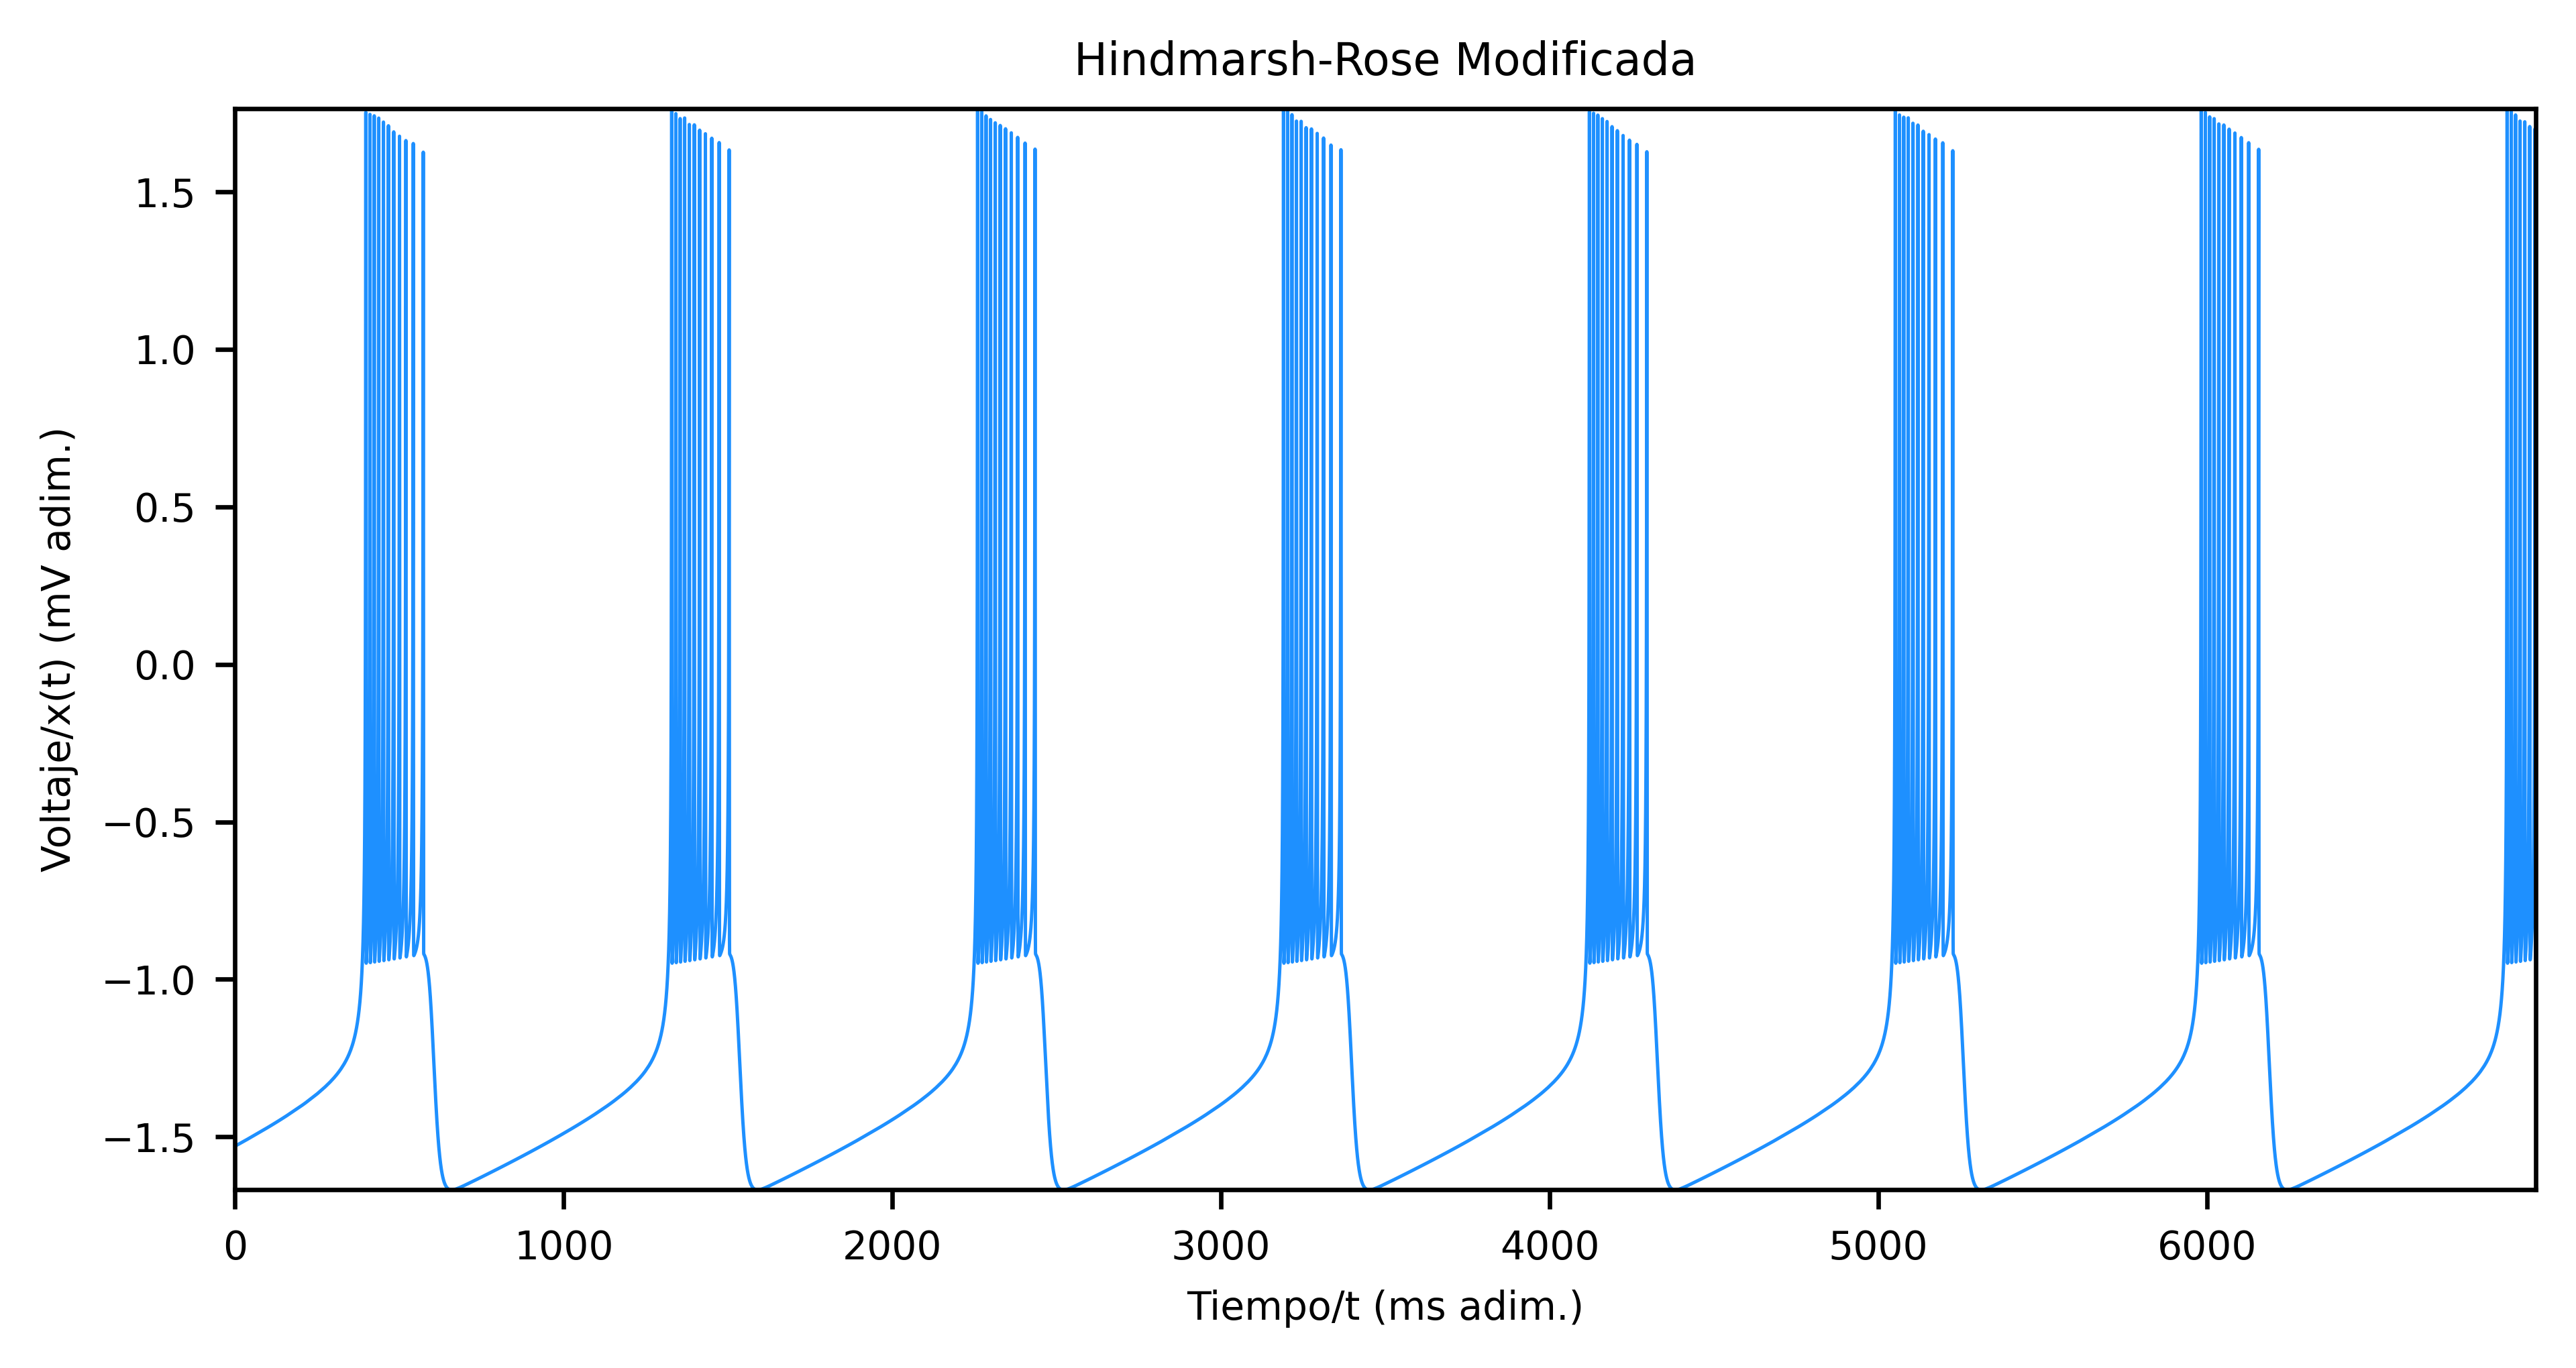
\includegraphics[width=\textwidth, height=\textheight, keepaspectratio]{hindmarsh-rose_modified}
\end{frame}


\begin{frame}{Modelo de sinapsis química gradual de Golowasch\footnote{J. Golowasch et al., \textit{Neural Comput.}, 1999.}: componente rápida}
    \textbf{Altas frec./\textit{spikes} de} $\boldsymbol{V_{\mathrm{pre}}}$ \\[0.8em]
    \scriptsize
    \begin{equation*}
        \boxed{\begin{aligned}
                \boldsymbol{I_{\mathrm{fast}}}           & = g_{\mathrm{fast}} \cdot \sigma_{\mathrm{fast}}(V_{\mathrm{pre}}) \cdot (V_{\mathrm{post}} - E_{\mathrm{syn}}) \\
                \sigma_{\mathrm{fast}}(V_{\mathrm{pre}}) & = \frac{1}{1 + \exp[ s_{\mathrm{fast}} \cdot (V_{\mathrm{fast}} - V_{\mathrm{pre}}) ]}
            \end{aligned}}
    \end{equation*}

    \begin{center}
        \setlength{\tabcolsep}{2pt}
        \begin{tabular}{|l|>{\raggedright\arraybackslash}m{3.4cm}|>{\raggedright\arraybackslash}m{2.6cm}|l|l|}
            \hline
            \textbf{Parámetro}  & \textbf{Descripción}                                                                  & \textbf{Escala con}                                                & \textbf{Unidad}    & \textbf{Valores interesantes}                     \\
            \hline
            \rowcolor{azulclaro}
            $g_{\mathrm{fast}}$ & Conductancia, controla amplitud                                                       & Rango $V_{\mathrm{post}}$ inv., rango $I_{\mathrm{fast}}$ objetivo & $\mathrm{\mu S}$   &                                                   \\
            \hline
            $E_{\mathrm{syn}}$  & Potencial de inversión, controla excitación/inhibición (fase/antifase) mediante signo & Rango $V_{\mathrm{post}}$                                          & mV                 & \makecell[l]{Alejado de rango $V_{\mathrm{post}}$ \\\\$>$ rango $V_{\mathrm{post}}$: excitación/fase\\$<$ rango $V_{\mathrm{post}}$: inhibición/antifase} \\
            \hline
            \rowcolor{azulclaro}
            $s_{\mathrm{fast}}$ & Pendiente sigmoide                                                                    & Rango $V_{\mathrm{pre}}$ inv.                                      & $\mathrm{mV}^{-1}$ & $s_{\mathrm{fast}} > s_{\mathrm{slow}}$           \\
            \hline
            $V_{\mathrm{fast}}$ & Umbral sigmoide                                                                       & Rango $V_{\mathrm{pre}}$                                           & mV                 & Valores altos $V_{\mathrm{pre}}$                  \\
            \hline
        \end{tabular}
    \end{center}
\end{frame}

\begin{frame}{Modelo de sinapsis química gradual de Golowasch\footnote{J. Golowasch et al., \textit{Neural Comput.}, 1999.}: componente lenta}
    \textbf{Bajas frec. de} $\boldsymbol{V_{\mathrm{pre}}}$ \\[0.8em]
    \small
    \begin{equation*}
        \boxed{\begin{aligned}
                \boldsymbol{I_{\mathrm{slow}}}              & = g_{\mathrm{slow}} \cdot m_{\mathrm{slow}} \cdot (V_{\mathrm{post}} - E_{\mathrm{syn}})                                      \\
                \boldsymbol{\frac{d m_{\mathrm{slow}}}{dt}} & \boldsymbol{= k_1 \cdot \sigma_{\mathrm{slow}}(V_{\mathrm{pre}}) \cdot (1 - m_{\mathrm{slow}}) - k_2 \cdot m_{\mathrm{slow}}} \\
                \sigma_{\mathrm{slow}}(V_{\mathrm{pre}})    & = \frac{1}{1 + \exp[ s_{\mathrm{slow}} \cdot (V_{\mathrm{slow}} - V_{\mathrm{pre}}) ]}
            \end{aligned}}
    \end{equation*}

    \begin{center}
        \setlength{\tabcolsep}{2pt}
        \begin{tabular}{|l|l|l|l|l|}
            \hline
            \textbf{Parámetro}  & \textbf{Descripción}              & \textbf{Escala con}           & \textbf{Unidad}           & \textbf{Valores interesantes}           \\
            \hline
            \rowcolor{azulclaro}
            $s_{\mathrm{slow}}$ & Pendiente sigmoide                & Rango $V_{\mathrm{pre}}$ inv. & $\mathrm{mV}^{-1}$        & $s_{\mathrm{fast}} > s_{\mathrm{slow}}$ \\
            \hline
            $V_{\mathrm{slow}}$ & Umbral sigmoide                   & Rango $V_{\mathrm{pre}}$      & mV                        & Valores bajos $V_{\mathrm{pre}}$        \\
            \hline
            \rowcolor{azulclaro}
            $k_1$               & Tasa apertura $m_{\mathrm{slow}}$ & Frec. de corte                & $\mathrm{\text{ms}}^{-1}$ &                                         \\
            \hline
            $k_2$               & Tasa cierre $m_{\mathrm{slow}}$   & Frec. de corte                & $\mathrm{\text{ms}}^{-1}$ &                                         \\
            \hline
        \end{tabular}
    \end{center}
\end{frame}


\begin{frame}{Modelo de sinapsis química gradual de Golowasch\footnote{J. Golowasch et al., \textit{Neural Comput.}, 1999.}}
    \begin{equation*}
        \boxed{I_{\mathrm{syn}} = I_{\mathrm{fast}} + I_{\mathrm{slow}}}
    \end{equation*}
    \vspace{0.8em}
    \begin{itemize}
        \item \textbf{\textit{Parameter sloppiness}} al afectar \textbf{todos} los params. a \textbf{amplitud}
              \vspace{1.5em}
        \item $I_{\mathrm{syn}}$ se inyecta en neurona \textbf{postsináptica} $\to$ una sinapsis \textbf{por dirección}
    \end{itemize}
\end{frame}



\begin{frame}{Función de evaluación de params.}
    Altas y bajas \textbf{frec. de} $\boldsymbol{V_{\mathrm{pre}}}$ como \textbf{ref. de corrientes (corrientes realistas)} $\to$ \textbf{filtro Butterworth paso bajo sobre} $\boldsymbol{V_{\mathrm{pre}}}$ (lib. KFR)
    \vspace{-1em}
    \begin{center}
        \begin{columns}[t]
            \begin{column}{0.48\textwidth}
                \begin{block}{Puntuación de forma}
                    \small
                    \textbf{Coeficiente de correlación de Pearson} normalizado en $[0, 1]$:
                    \begin{itemize}
                        \item \textbf{Antifase} $\to$ \textbf{correlación}
                        \item \textbf{Fase} $\to$ \textbf{correlación negativa}
                    \end{itemize}
                \end{block}
            \end{column}
            \begin{column}{0.48\textwidth}
                \begin{block}{Puntuación de rango}
                    \small
                    \begin{equation*}
                        \mathrm{score}_{\mathrm{rango}} = 1 - \frac{\frac{1}{2}(|\Delta I_{\min}| + |\Delta I_{\max}|)}{d_{\max}}
                    \end{equation*}
                    \begin{itemize}
                        \item En $\boldsymbol{[-\infty, 1]}$, normalmente $\ge 0$
                        \item \textbf{Extremos objetivo}:
                              \begin{itemize}
                                  \small
                                  \item Si \textbf{una componente de corriente}: usuario
                                  \item Si \textbf{ambas}: usuario, escalados con ref. (componente rápida con amplitud; lenta, amplitud + offset)
                              \end{itemize}
                    \end{itemize}
                \end{block}
            \end{column}
        \end{columns}
        \vspace{0.8em}
        \fcolorbox{azulprimario}{azulclaro}{Puntuación = media}
    \end{center}
\end{frame}


\begin{frame}{\textit{Bayesian Optimization} (BO)}
    Construye \textbf{GP} (\textbf{modelo subrogado}) de objetivo (lib. \textbf{Limbo}):
    \vspace{1em}
    \begin{itemize}
        \item \textbf{\textit{Kernel} SE-ARD} $\to$ anti-\textit{parameter sloppiness}
        \item \textbf{Hiperparams. reoptimizados con Rprop}
        \item \textbf{Adquisición \textit{EI} maximizada con Subplex} (lib. NLOpt) $\to$ \textbf{equilibrio exploración-explotación} (\textit{jitter})
        \item \textbf{Muestras iniciales LHS} $\to$ cobertura \textbf{uniforme}
    \end{itemize}
\end{frame}


\begin{frame}{Configs. de espacio de búsqueda}
    \small
    \begin{columns}[t]
        \begin{column}{0.48\textwidth}
            \textbf{Rangos dinámicos adaptados:}
            \begin{itemize}
                \item[] BO con params. en $\boldsymbol{[0, 1]}$ $\to$ \textbf{desnormalización} previo uso
                \item[] \textbf{Rangos de desnormalización}: calculados según lo visto y $g_{\mathrm{fast/slow}}$ con extremos de los otros rangos y de $I_{\mathrm{fast/slow}}$ objetivo
            \end{itemize}
        \end{column}
        \begin{column}{0.48\textwidth}
            \textbf{Medidas anti-\textit{parameter sloppiness}:}
            \begin{itemize}
                \item \textit{Kernel} \textbf{SE-ARD} $\to$ escala de longitud \textbf{por param.}
                \item \textbf{Reparametrización} $\boldsymbol{R = k_2/k_1}$ $\to$ desacoplamiento entre \textbf{cinética} y \textbf{equilibrio apertura-cierre}
                      \begin{equation*}
                          m_{\mathrm{slow}}^{\infty} = \frac{\sigma_{\mathrm{slow}}(V_{\mathrm{pre}})}{\sigma_{\mathrm{slow}}(V_{\mathrm{pre}}) + \boldsymbol{R}}
                      \end{equation*}
                      \vspace{-0.5em}
                \item \textbf{Escala logarítmica} en $\boldsymbol{g}$, $\boldsymbol{k_1}$, $\boldsymbol{R}$ ($k_2$) $\to$ reducción de \textbf{anisotropía} del espacio (además abarcan \textbf{varios órdenes} de magnitud)
            \end{itemize}
        \end{column}
    \end{columns}
\end{frame}


\begin{frame}{Escalado de señal presináptica de Reyes-Sanchez\footnote{M. Reyes-Sanchez et al., \textit{Neuroinformatics}, 2020.}}
    Neurona \textbf{HR} en \textbf{unidades adimensionales} de amplitud y tiempo; \textbf{viva}, en \textbf{reales}
    \vspace{-1em}
    \begin{columns}[t]
        \begin{column}{0.48\textwidth}
            \begin{block}{Escalado de amplitud}
                \vspace{-1em}
                \begin{equation*}
                    \begin{aligned}
                        \mathrm{factor} & = \frac{\Delta V_{\mathrm{model}}}{\Delta V_{\mathrm{real}}}               \\
                        \mathrm{offset} & = V_{\mathrm{model,}\min} - (V_{\mathrm{real,}\min} \cdot \mathrm{factor}) \\
                        \\ \boldsymbol{V_{\mathrm{escalado}}} & \boldsymbol{= V_{\mathrm{real}} \cdot \mathrm{factor} + \mathrm{offset}}
                    \end{aligned}
                \end{equation*}
            \end{block}
        \end{column}
        \begin{column}{0.48\textwidth}
            \begin{block}{Escalado temporal}
                Buscar \textbf{mayor} $\boldsymbol{dt}$ \textbf{estable} del modelo tal que \textbf{núm. de puntos por periodo de \textit{burst}} sea \textbf{múltiplo entero (factor de submuestreo) cercano a núm. de muestras de la otra neurona}
            \end{block}
        \end{column}
    \end{columns}
    \vspace{1em}
    \textbf{Programa} para \textbf{precalcular} datos de neurona \textbf{modelo} $\to$ \textbf{no se repite}
\end{frame}


\begin{frame}{Implementación \textit{offline}: esquema}
    \centering
    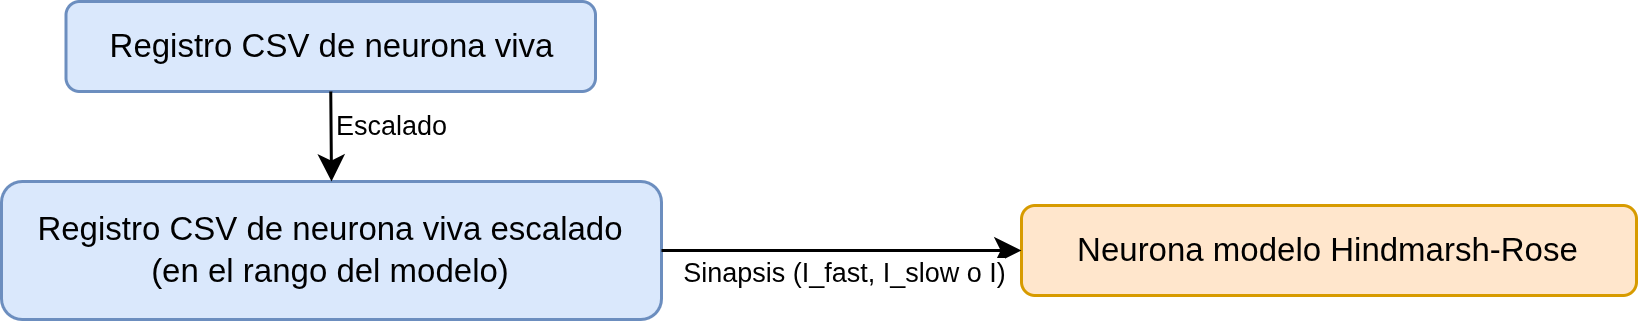
\includegraphics[width=\textwidth, height=\textheight, keepaspectratio]{esquema_neuronas_offline}
\end{frame}


\begin{frame}{Implementación \textit{offline}}
    \begin{itemize}
        \item \textbf{Sin esperas} de tiempo real $\to$ \textbf{veloz}
        \item Registro de \textbf{neurona PD de ganglio estomatogástrico de crustáceo} (\textit{bursting} de \textbf{CPG})
        \item Integrador \textbf{Runge-Kutta} $\to$ equilibrio \textbf{eficiencia-coste}
        \item \textbf{Evals. deterministas} (mismo interval. de reg. y reinicio de vars.) $\to$ \textbf{ruido fijo y reducido} en BO
        \item Lib. de modelos \textbf{Neun} $\to$ fácil cambio de modelos
    \end{itemize}
\end{frame}


\begin{frame}{Implementación \textit{offline}: configs. usuario}
    \begin{itemize}
        \item Núm. \textbf{muestras iniciales + iteraciones = evals.}
        \item \textbf{Tiempos de estabilización (modelos) y eval.}
        \item \textbf{Frec. de corte}
        \item \textbf{Componentes de corriente} a optimizar y su \textbf{rango objetivo}
        \item Búsqueda de \textbf{fase o antifase}
    \end{itemize}
\end{frame}


\begin{frame}{Implementación \textit{online}: esquema}
    \centering
    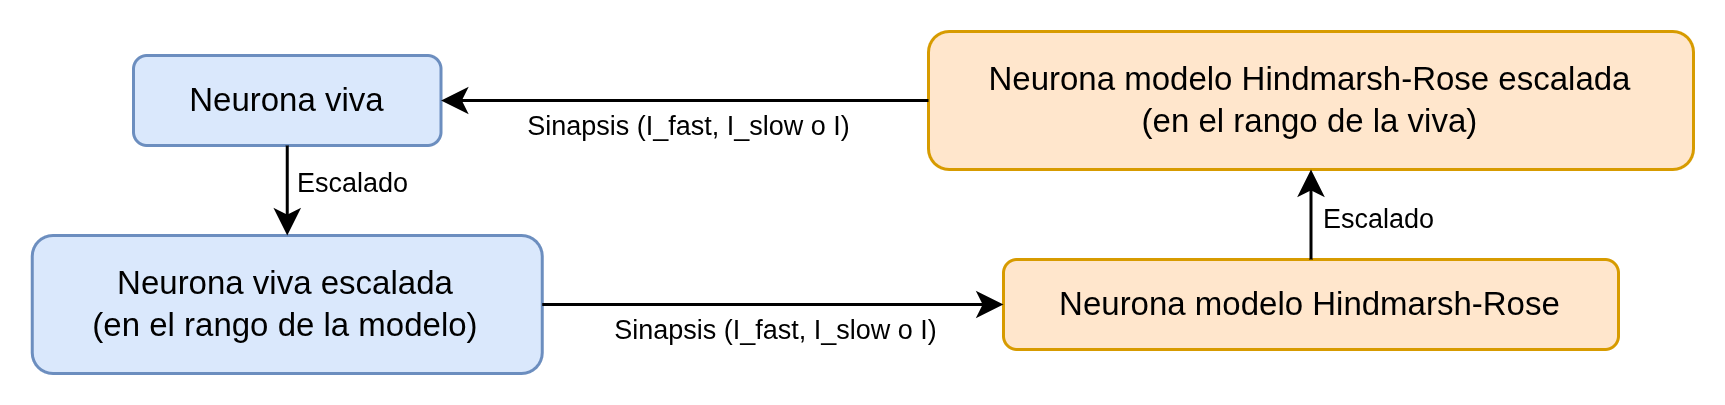
\includegraphics[width=\textwidth, height=\textheight, keepaspectratio]{esquema_neuronas_online}
\end{frame}


\begin{frame}{Implementación \textit{online}}
    \begin{itemize}
        \item Módulo \textbf{RTXI 2.3} (lab.)
        \item \textbf{Módulo sináptico}, no solo parametriza
        \item \textbf{Implementación propia de modelo} para calcular solo corrientes \textbf{seleccionadas} $\to$ \textbf{eficiencia}, crítica en \textbf{tiempo real}
        \item $\boldsymbol{dt}$ \textbf{pequeño, propio y sin submuestreo/escalado temporal}. Estable porque $m_{\mathrm{slow}}$ es lineal en su EDO.
        \item \textbf{Evals. no deterministas} (dist. interval.) $\to$ \textbf{ruido moderado y optimizable} y \textbf{\textit{jitter} bajo} (no explotar ruido) en BO
    \end{itemize}
\end{frame}

\begin{frame}{Implementación \textit{online}: hilos}
    \textbf{Tres} hilos:
    \begin{itemize}
        \item \textbf{RT (operaciones ligeras)}: \textbf{calcula corrientes} y \textbf{recolecta señales} para NRT, coordinándose con \textbf{variables atómicas} y \textbf{\textit{double buffering}} $\to$ \textbf{sin bloqueos}
        \item \textbf{NRT (operaciones pesadas)}: \textbf{optimización}, \textbf{reservas de memoria}...
        \item \textbf{GUI}
    \end{itemize}
\end{frame}


\begin{frame}{Implementación \textit{online}: esquema de módulos para dos neuronas modelo}
    \centering
    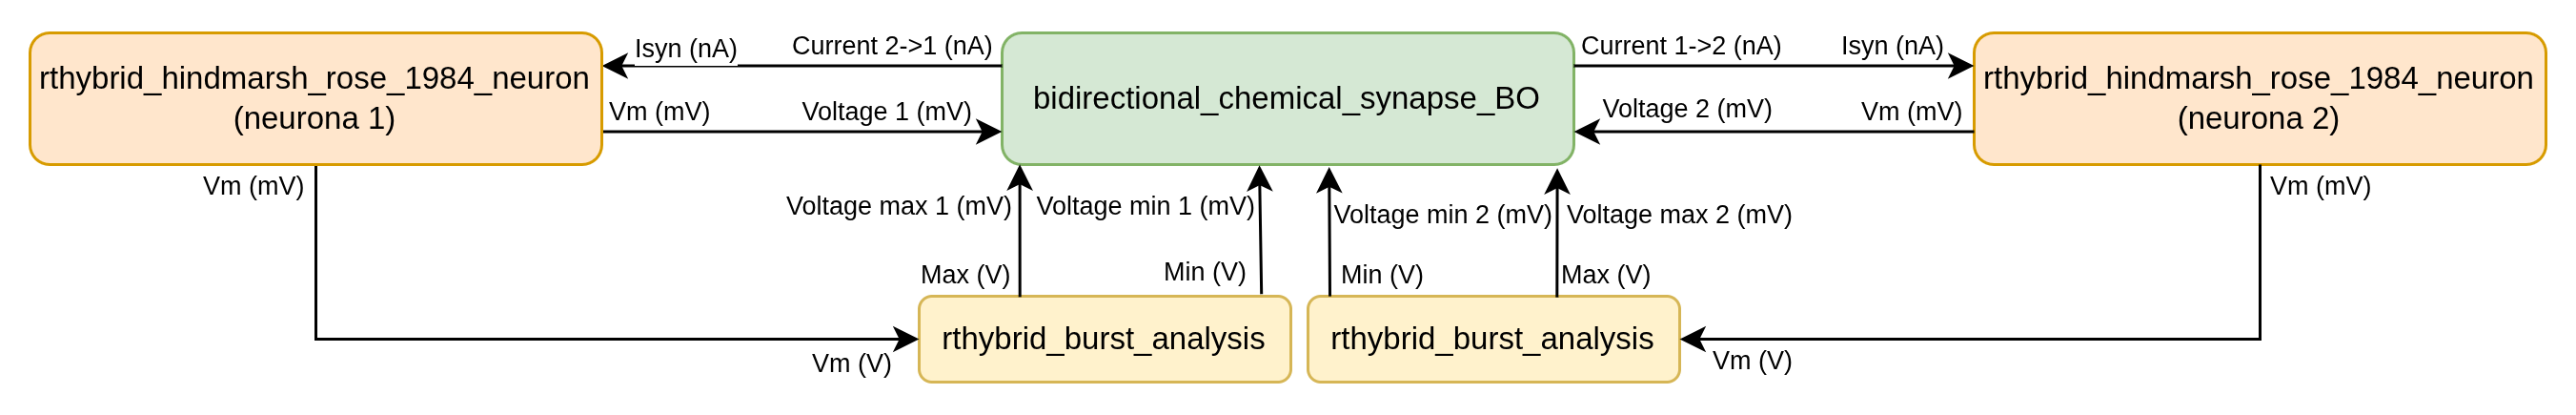
\includegraphics[width=\textwidth, height=\textheight, keepaspectratio]{esquema_modulos_online_modelo}
\end{frame}


\begin{frame}{Implementación \textit{online}: esquema de módulos para neurona modelo + viva}
    \centering
    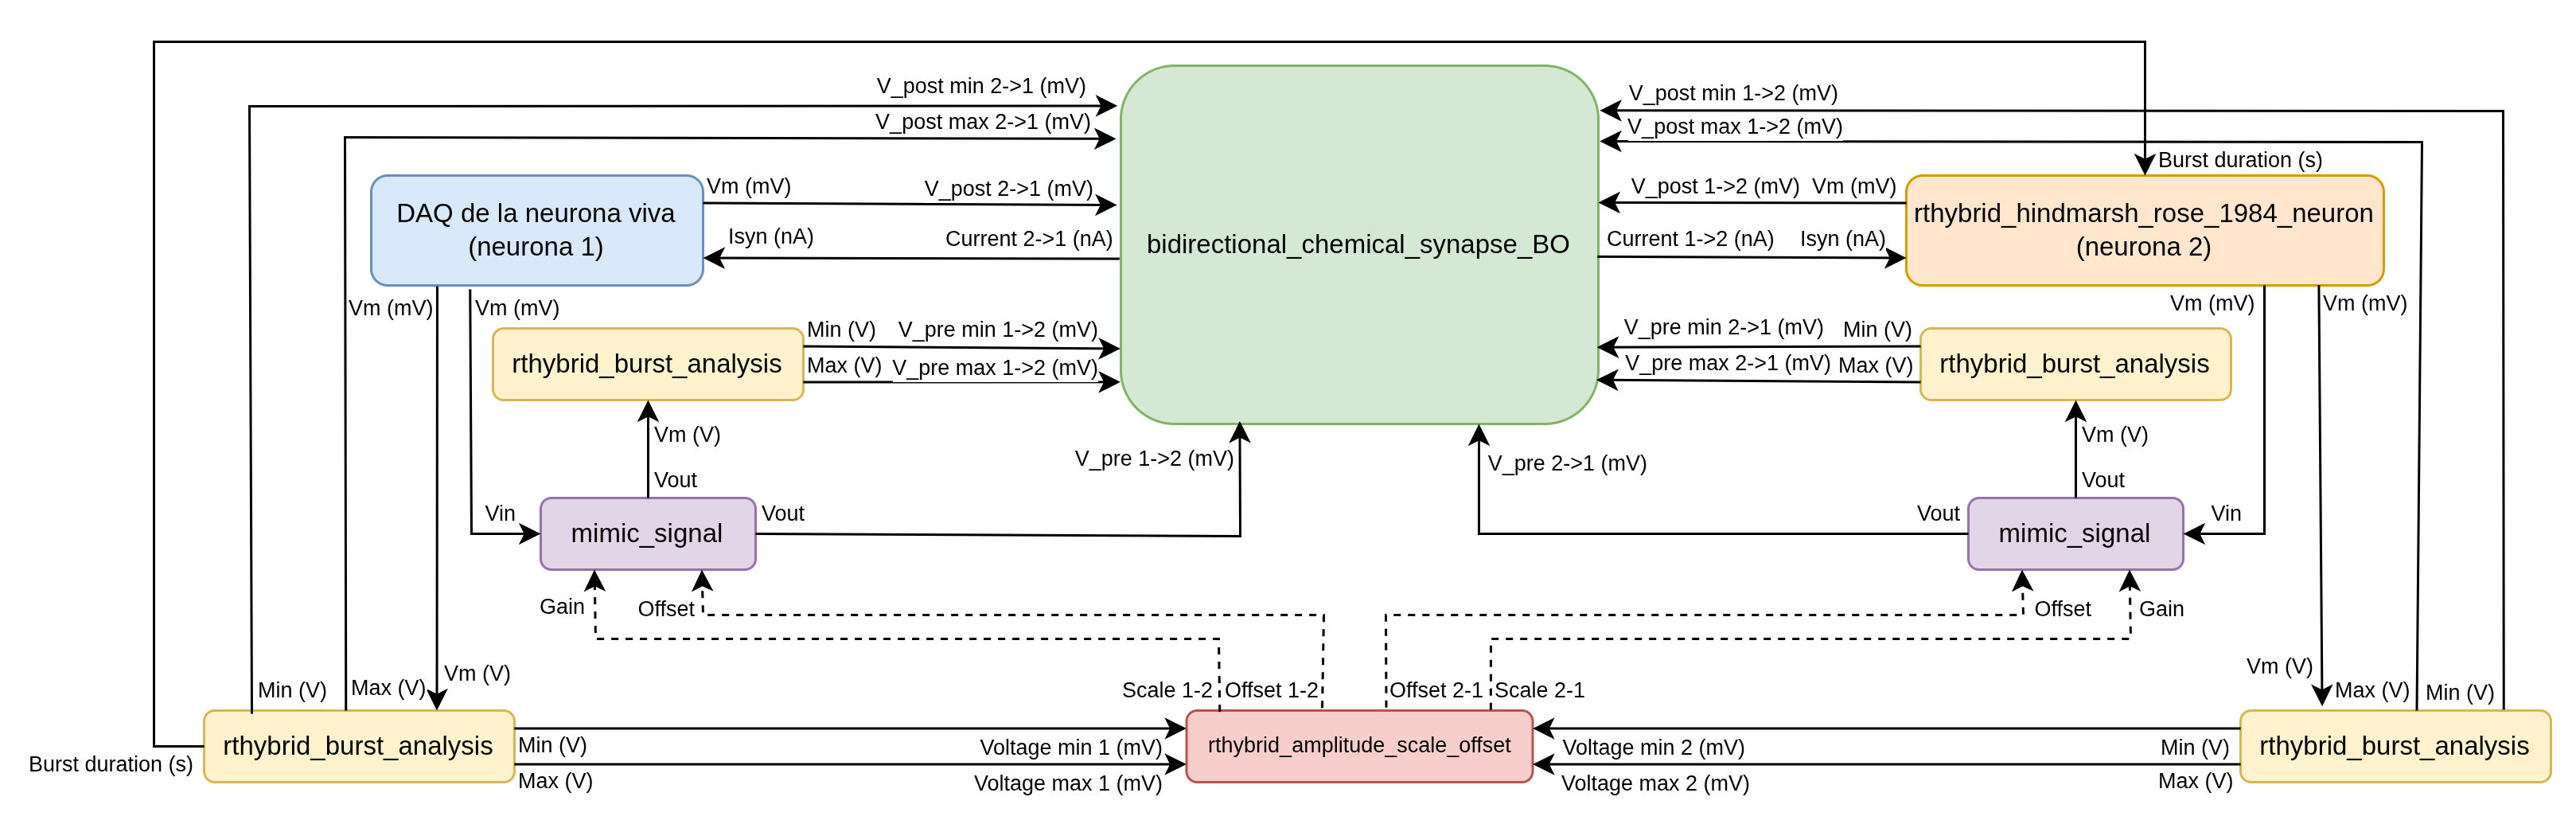
\includegraphics[width=\textwidth, height=\textheight, keepaspectratio]{esquema_modulos_online_viva}
\end{frame}


\section{Resultados}



\begin{frame}{Resultados implementación \textit{offline}: configs.}
    \begin{itemize}
        \item $\boldsymbol{I_{\mathrm{fast}}}$ \textbf{+} $\boldsymbol{I_{\mathrm{slow}}}$
        \item \textbf{50 muestras iniciales + 350 iteraciones = 400 evals.} $\to$ \textbf{suficiente} y \textbf{no excesivo}
        \item \textbf{Evals.} de $\boldsymbol{\sim 5}$ \textbf{\textit{bursts}}
        \item Promedio de \textbf{20 ejecuciones} $\to$ \textbf{rigurosidad estadística}
        \item \textbf{Rangos de corrientes objetivo suficientes} (fase/antifase) y \textbf{no excesivos}
    \end{itemize}
\end{frame}


\begin{frame}{Resultados implementación \textit{offline}: convergencia para antifase}
    \centering
    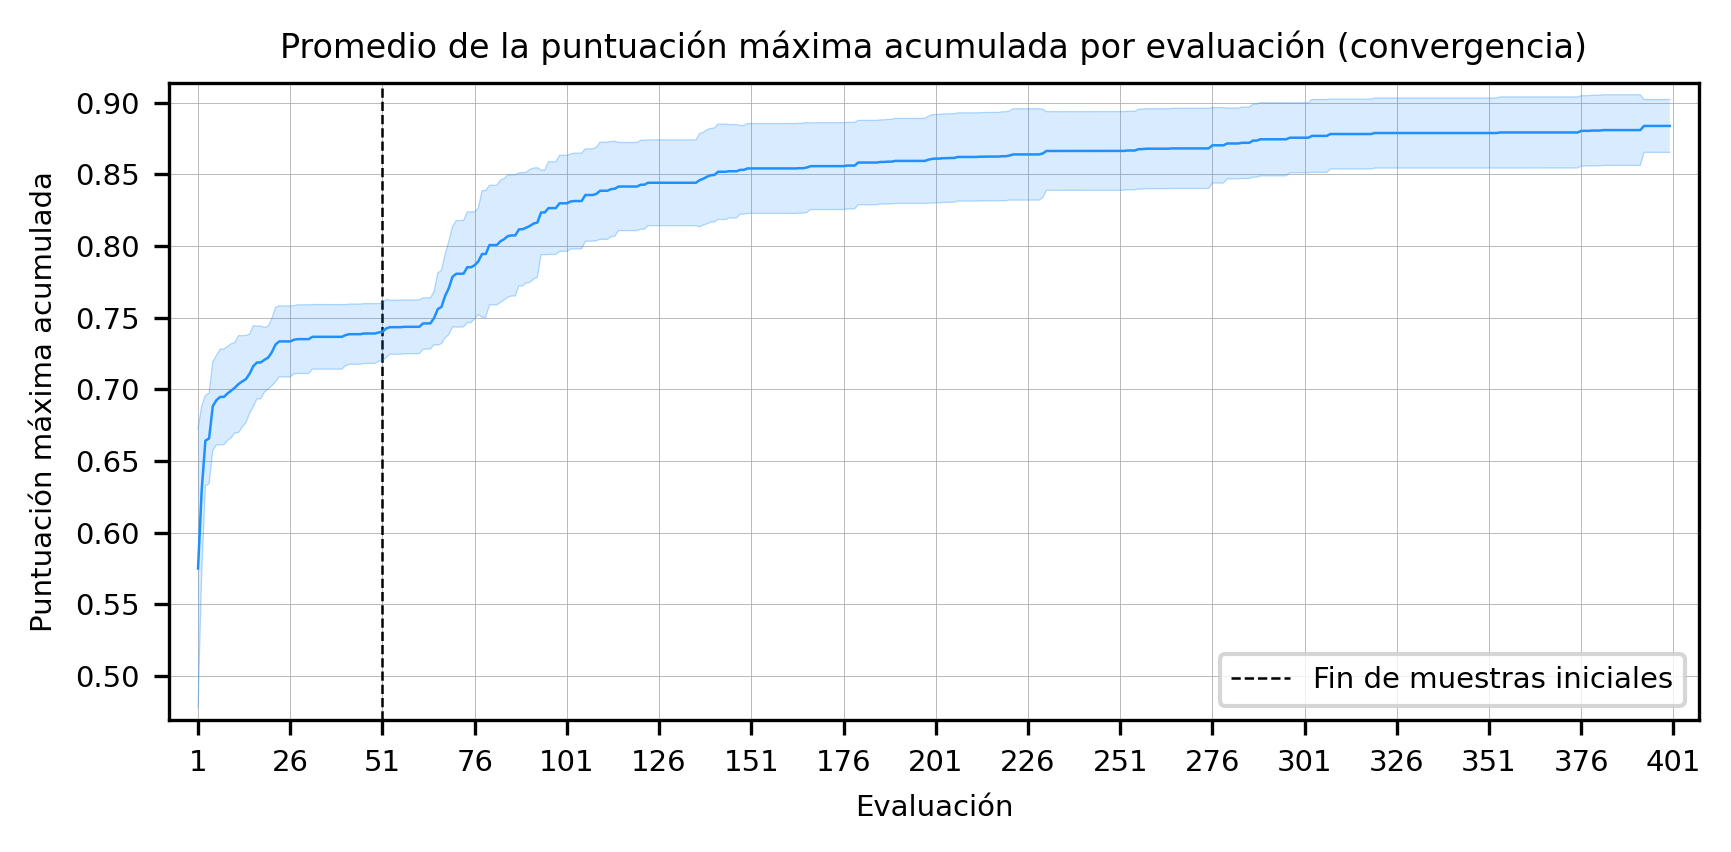
\includegraphics[width=\textwidth, height=\textheight, keepaspectratio]{bo_history_offline_syn_i_antiphase_acc_max}
\end{frame}


\begin{frame}{Resultados implementación \textit{offline}: convergencia para fase}
    \centering
    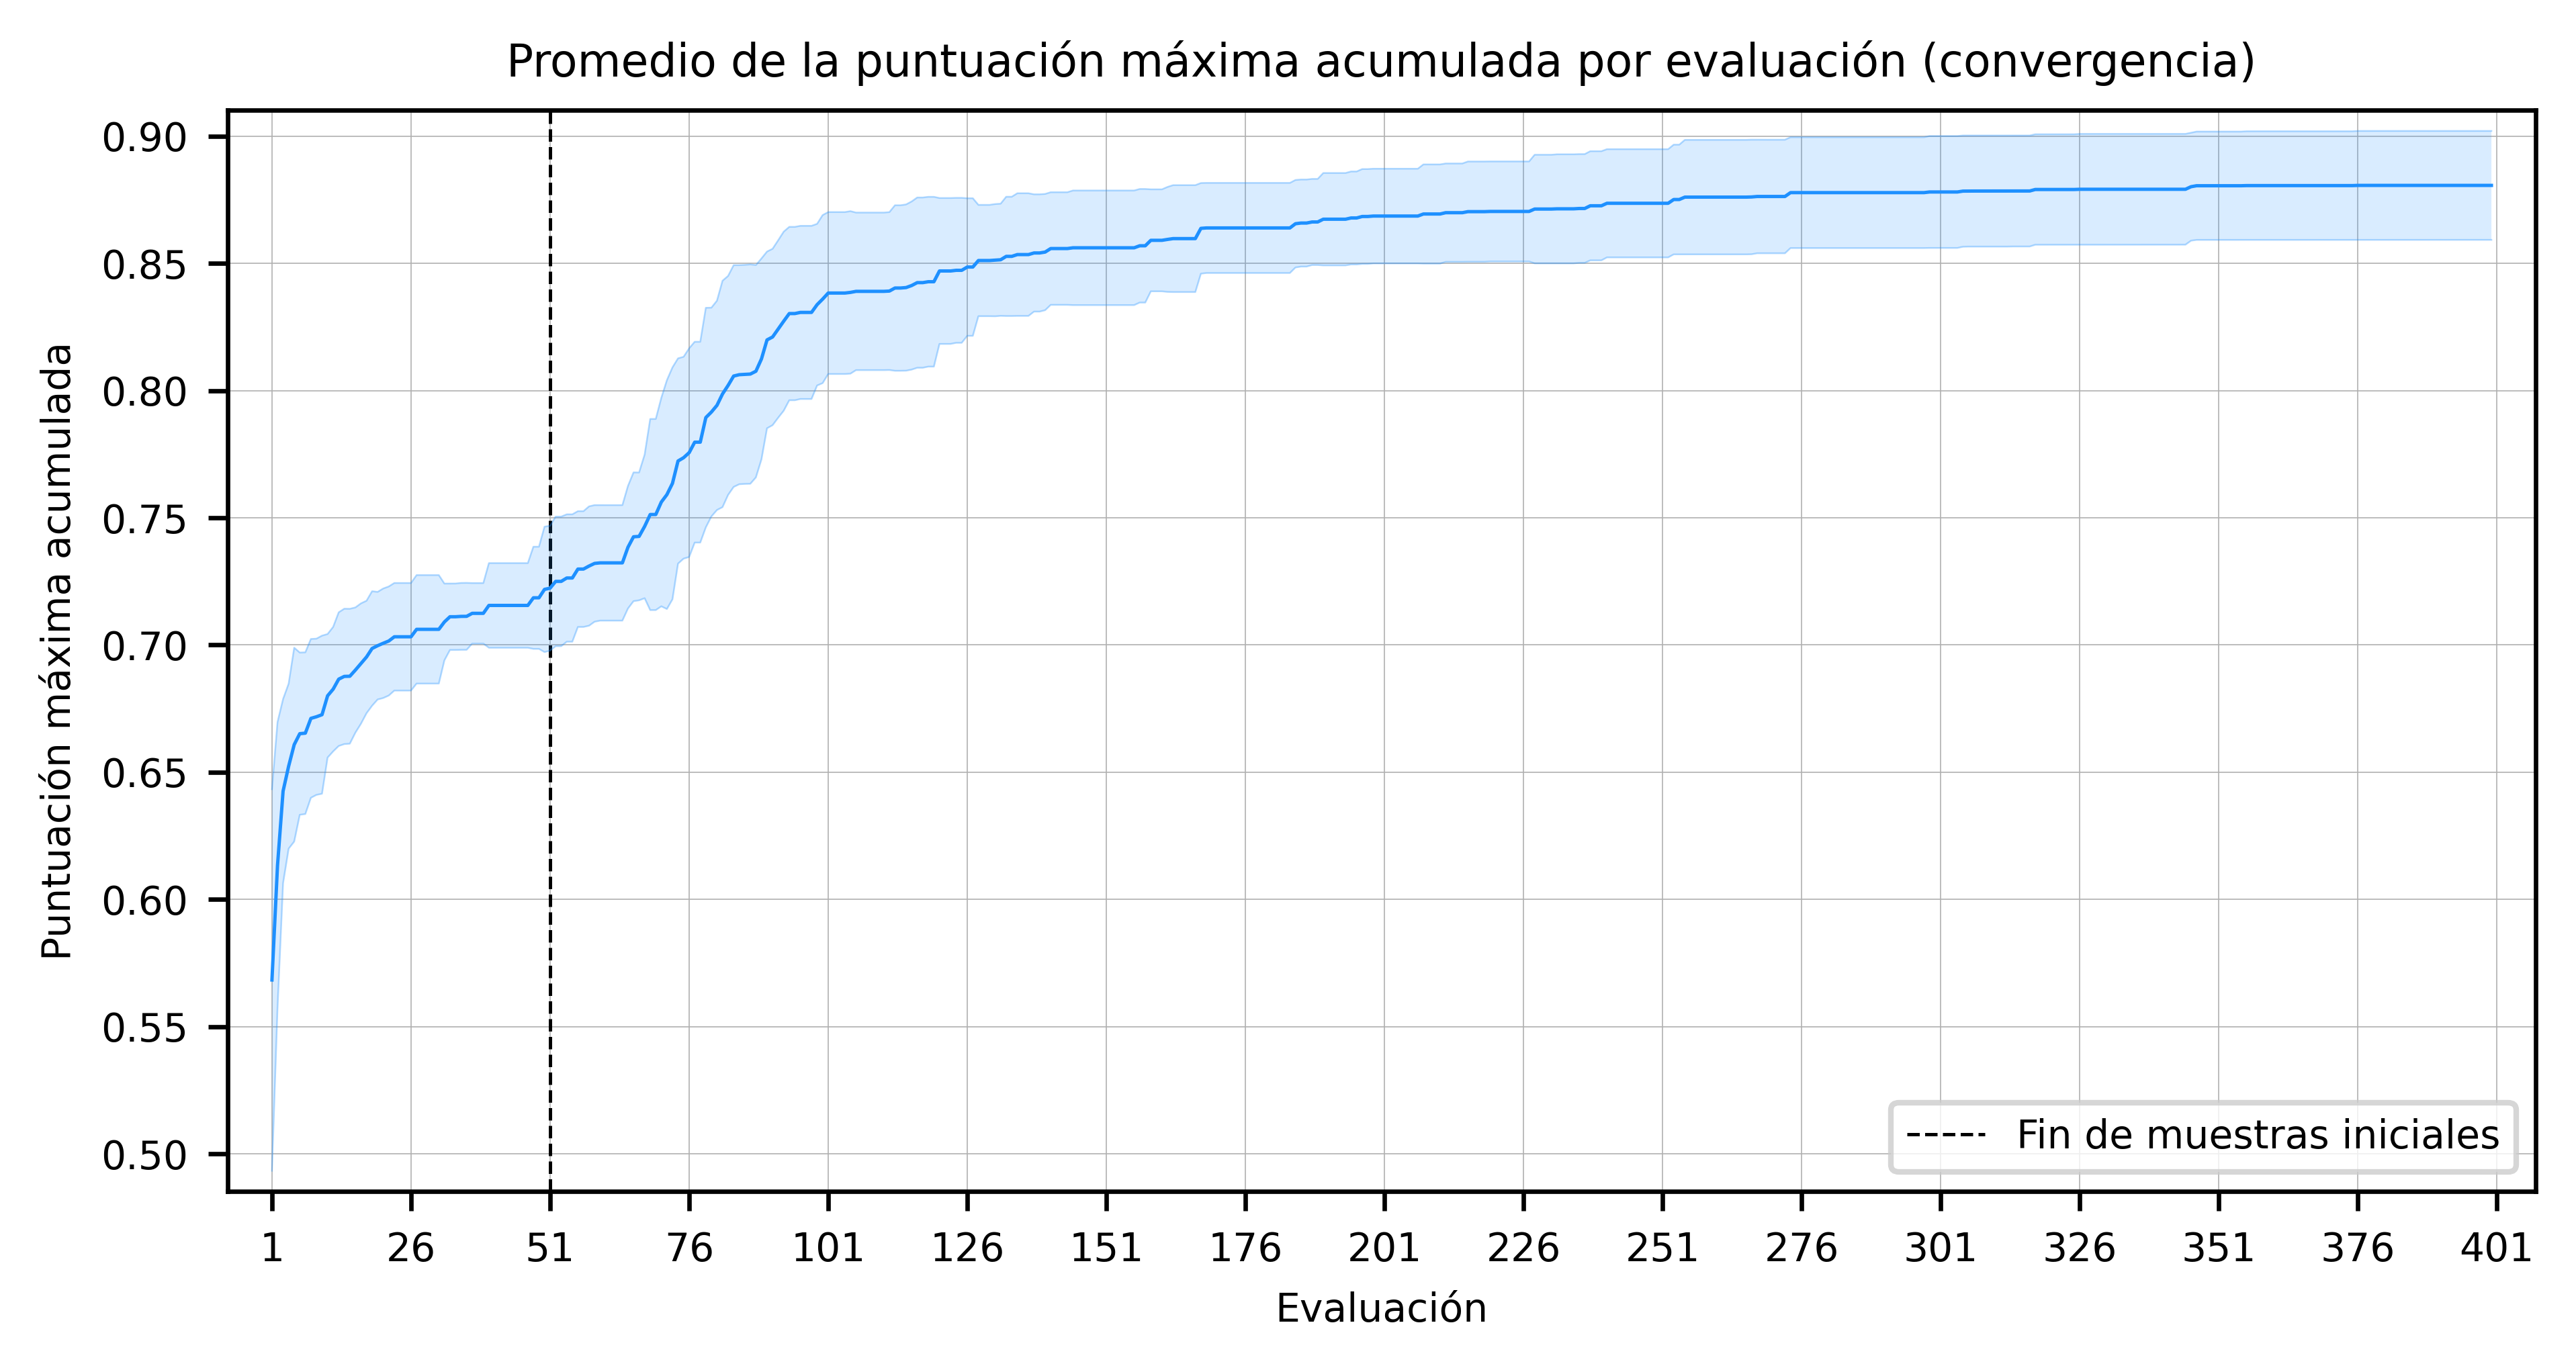
\includegraphics[width=\textwidth, height=\textheight, keepaspectratio]{bo_history_offline_syn_i_phase_acc_max}
\end{frame}


\begin{frame}{Resultados implementación \textit{offline}: puntuaciones para antifase}
    \centering
    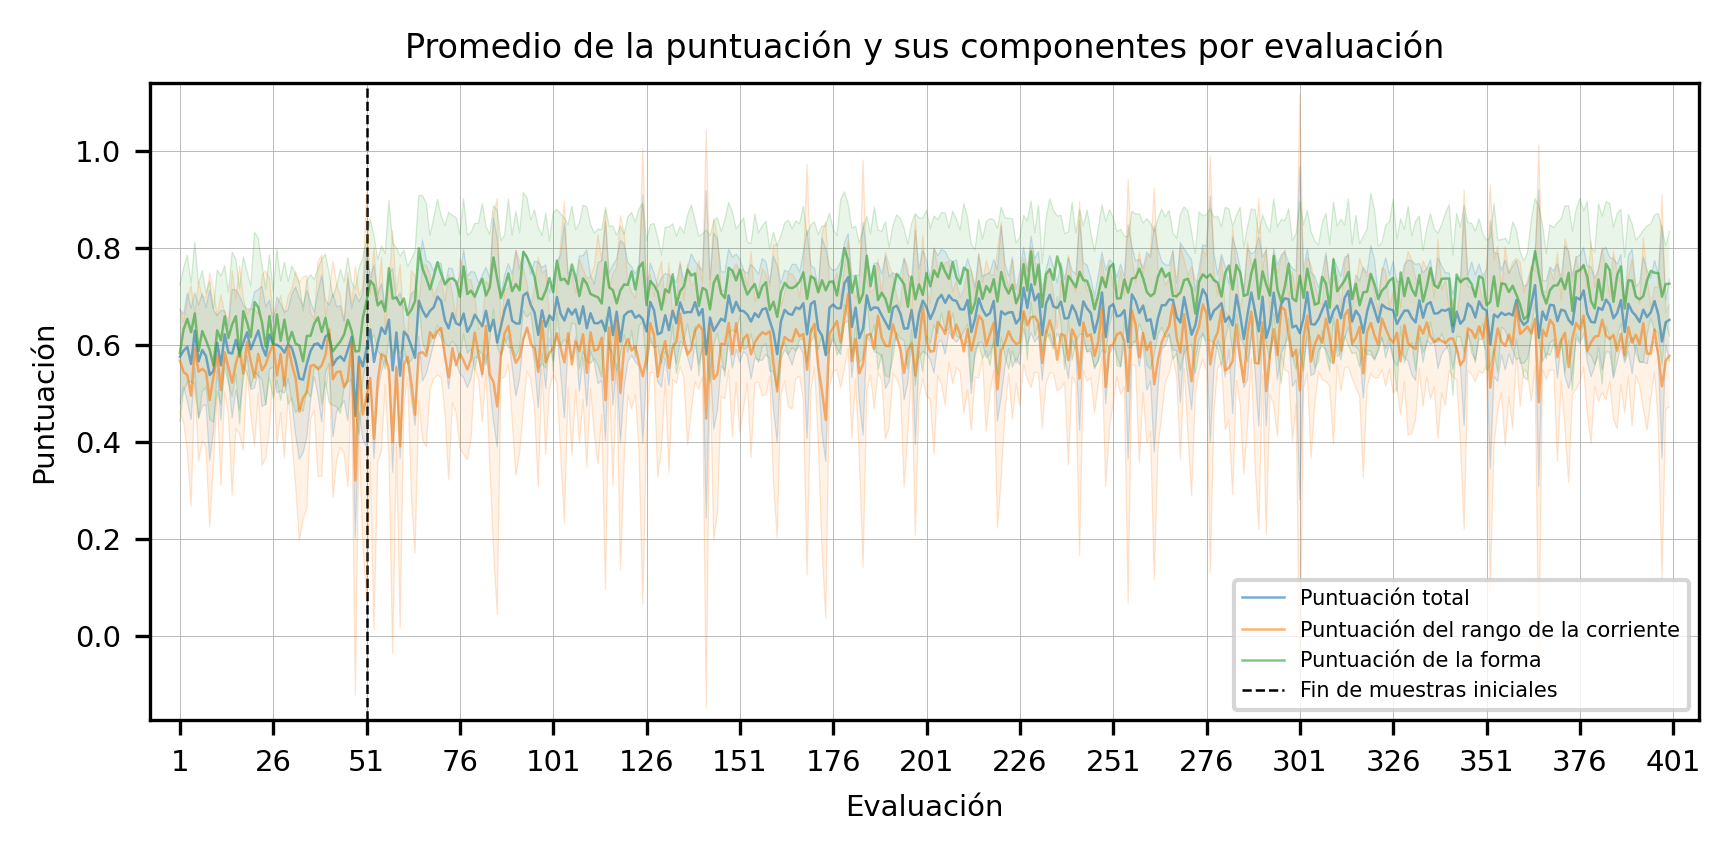
\includegraphics[width=\textwidth, height=\textheight, keepaspectratio]{bo_history_offline_syn_i_antiphase_avg_scores}
\end{frame}


\begin{frame}{Resultados implementación \textit{offline}: puntuaciones de una ejecución para antifase}
    \centering
    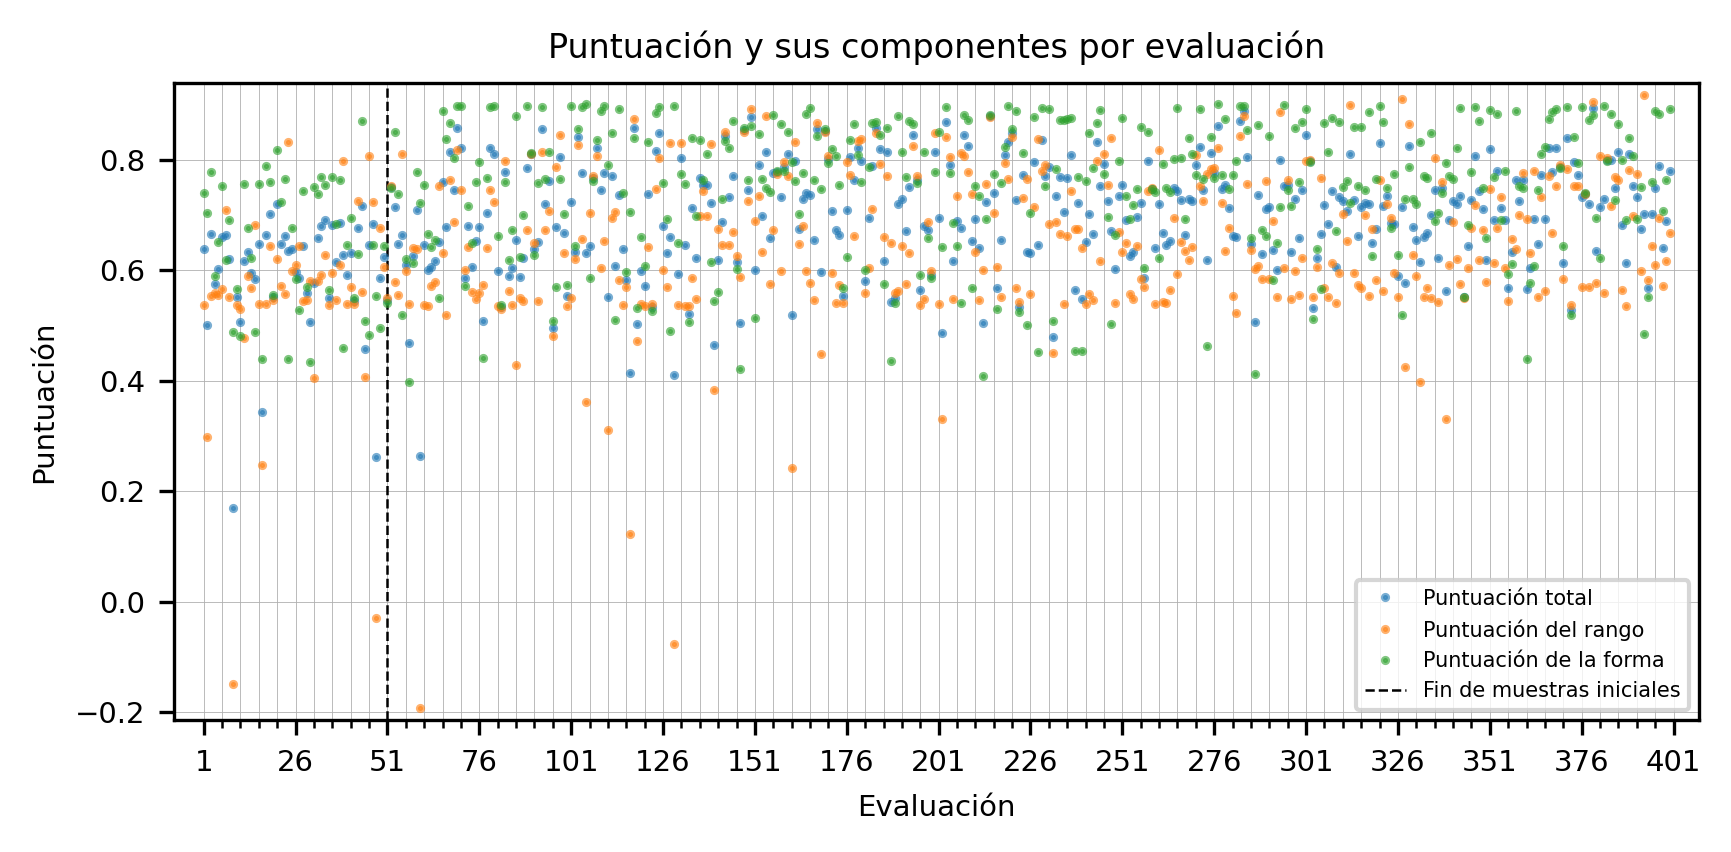
\includegraphics[width=\textwidth, height=\textheight, keepaspectratio]{bo_history_offline_syn_i_antiphase_scores}
\end{frame}


\begin{frame}{Resultados implementación \textit{offline}: dinámica result. para antifase}
    \centering
    \vspace{-0.3em}
    \begin{columns}
        \begin{column}{0.6\textwidth}
            \centering
            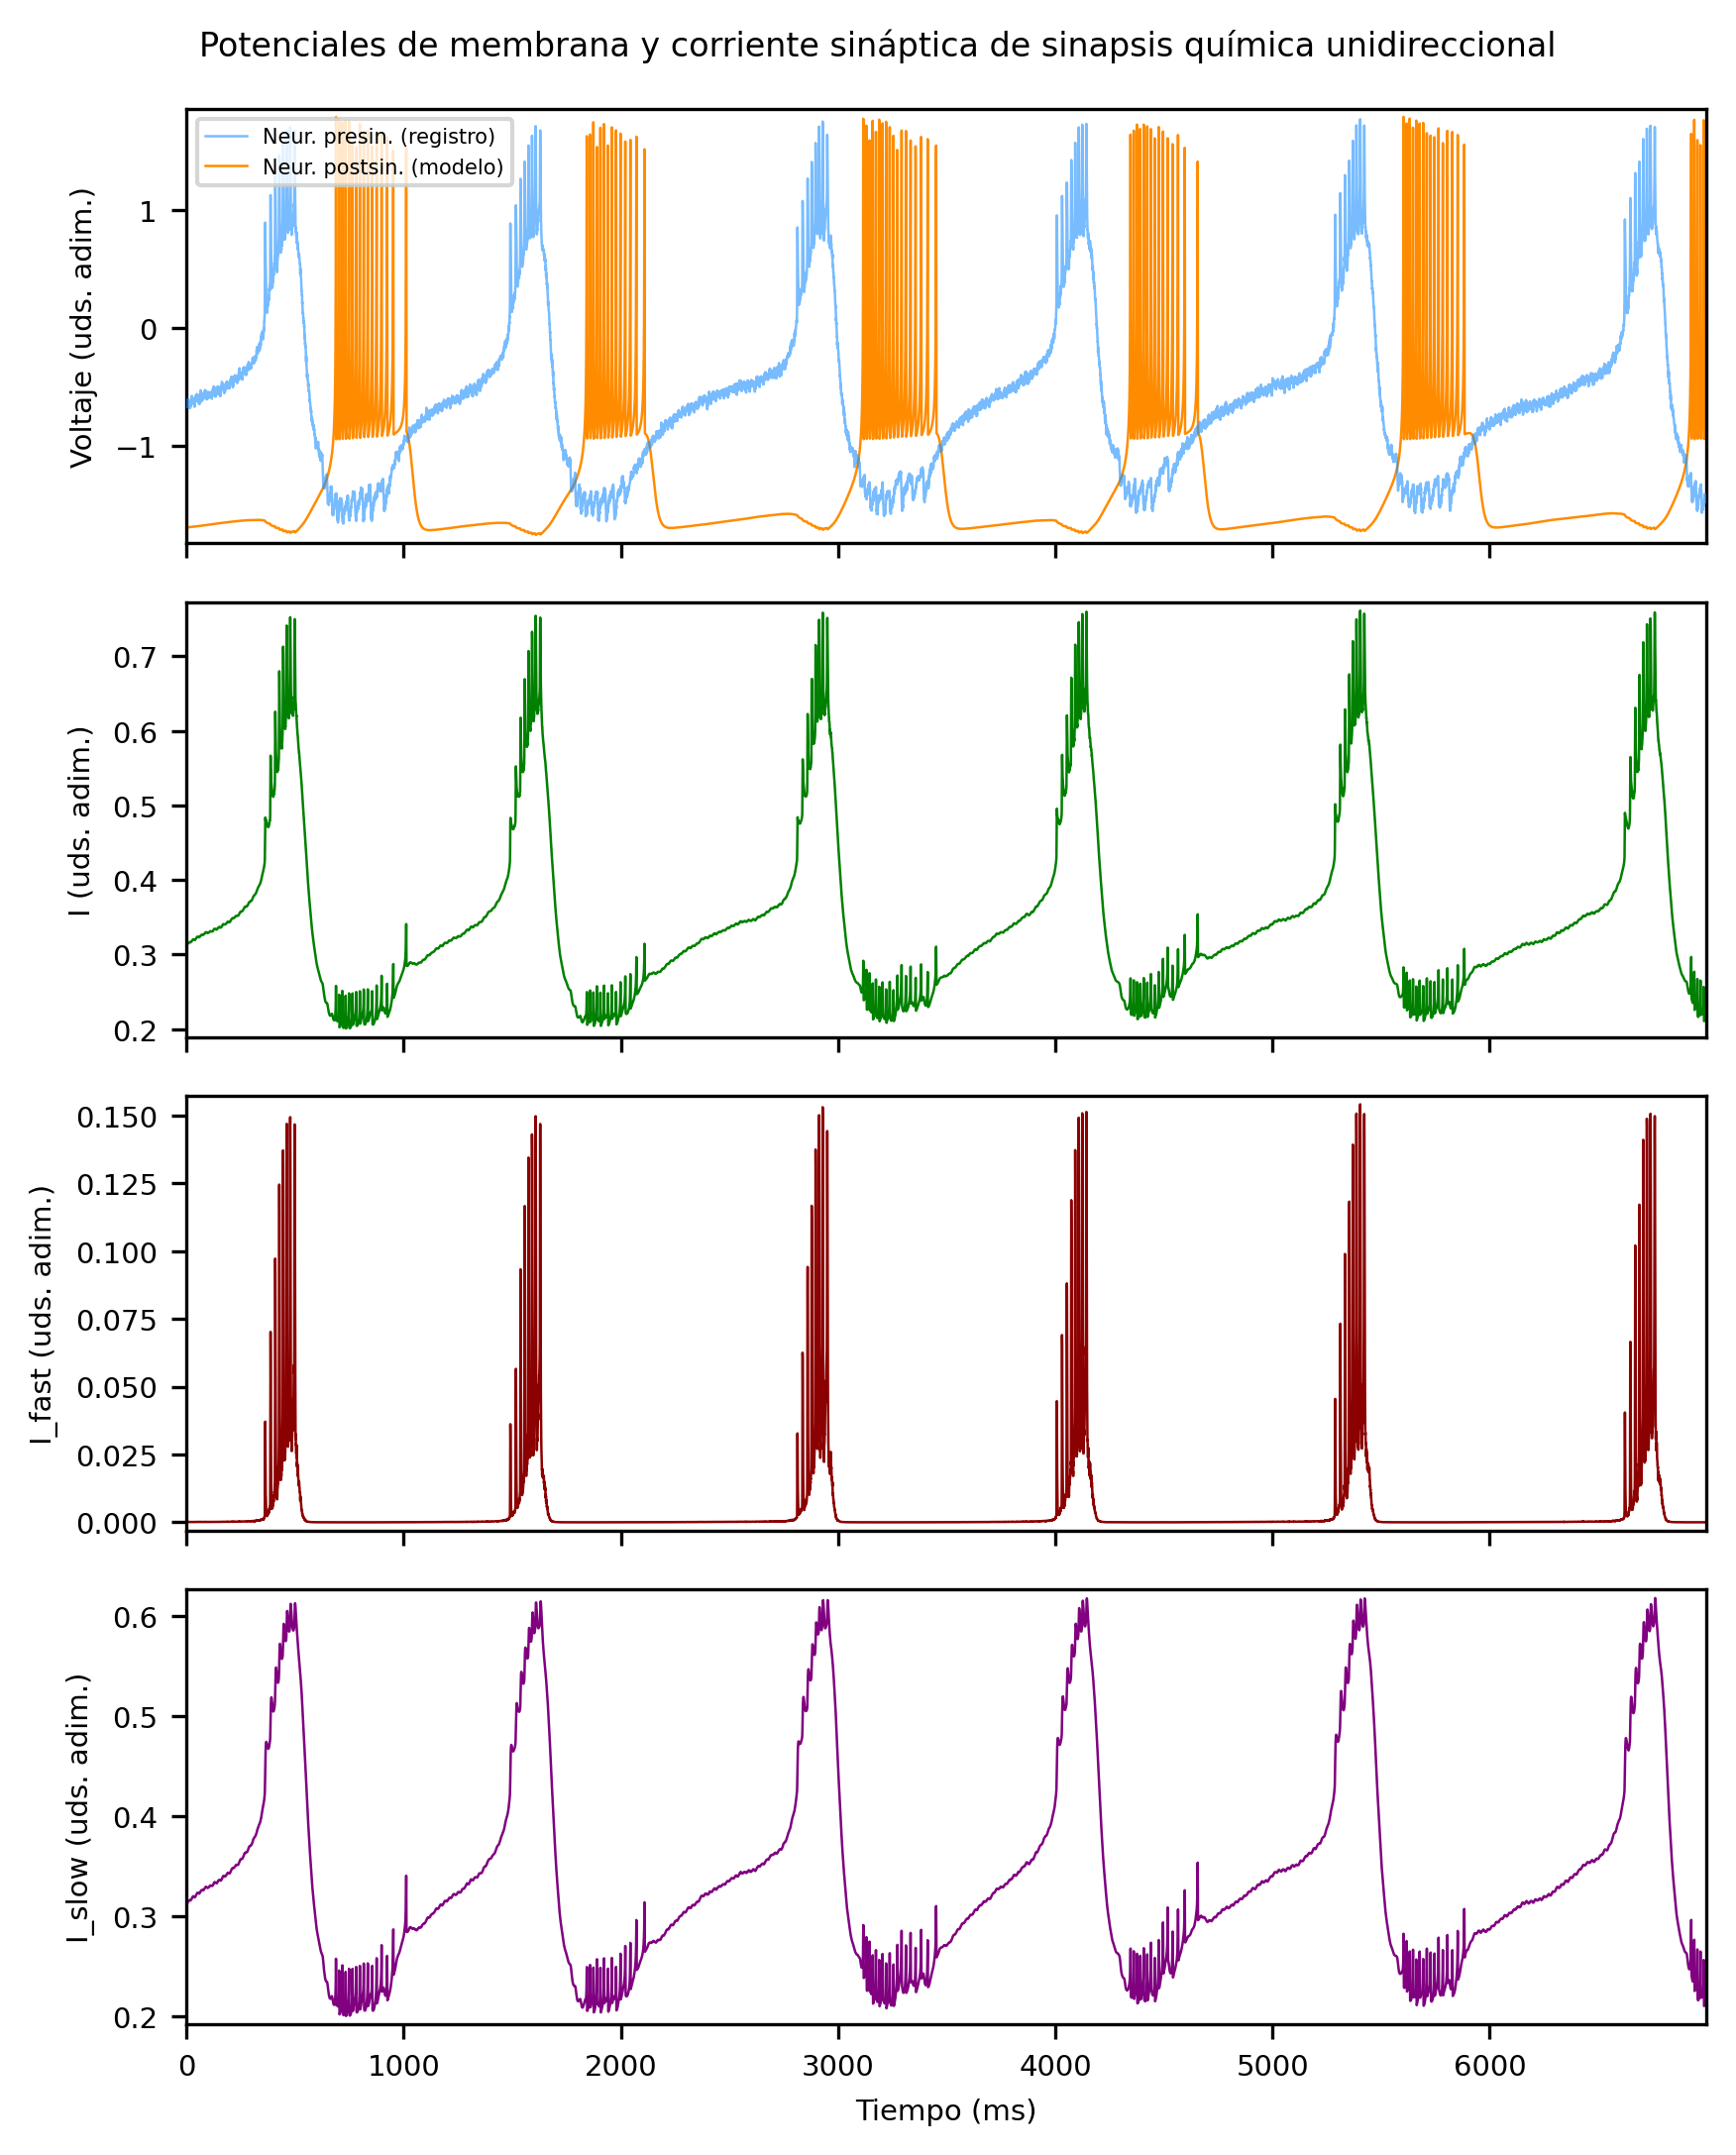
\includegraphics[height=0.92\textheight, keepaspectratio]{offline_syn_i_antiphase}
        \end{column}
        \begin{column}{0.4\textwidth}
            \textbf{Rango de corriente objetivo}:
            \begin{itemize}
                \item[] $\boldsymbol{[0{,}2; 0{,}8]}$ u. a.
            \end{itemize}
        \end{column}
    \end{columns}
\end{frame}


\begin{frame}{Resultados implementación \textit{offline}: dinámica result. para fase}
    \centering
    \vspace{-0.3em}
    \begin{columns}
        \begin{column}{0.6\textwidth}
            \centering
            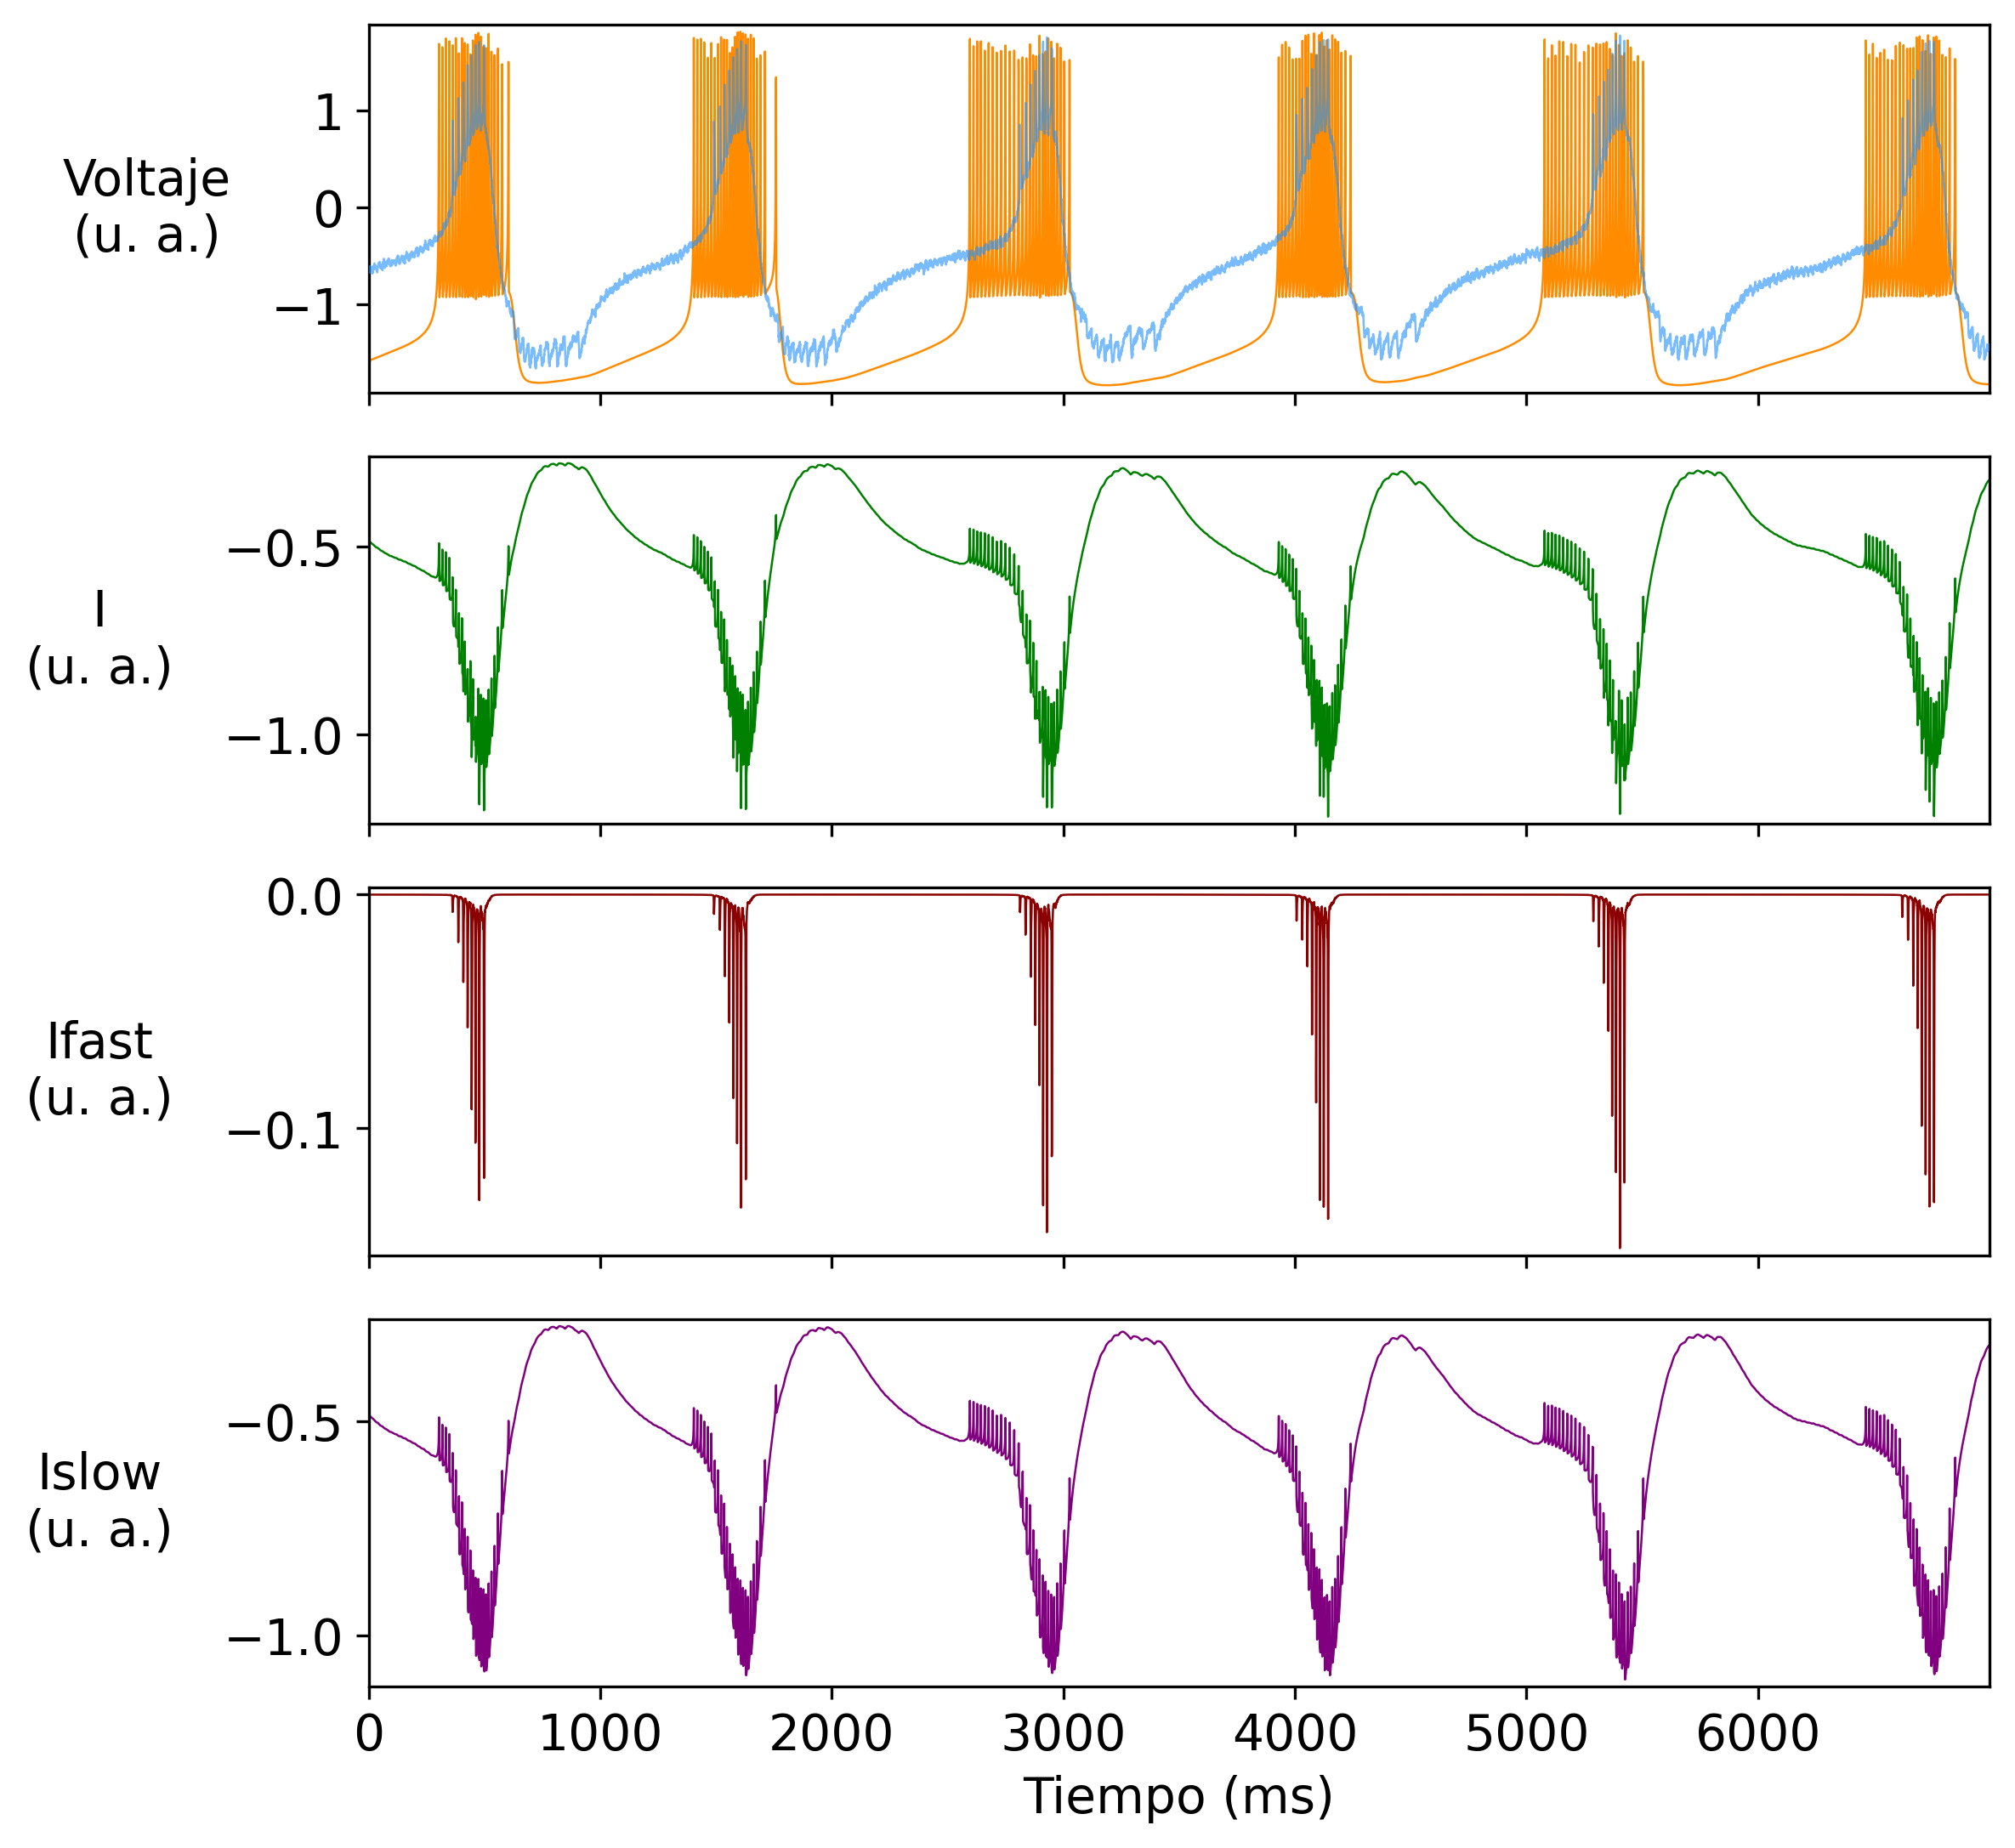
\includegraphics[height=0.92\textheight, keepaspectratio]{offline_syn_i_phase}
        \end{column}
        \begin{column}{0.4\textwidth}
            \textbf{Rango de corriente objetivo}:
            \begin{itemize}
                \item[] $\boldsymbol{[-1{,}4; -0{,}4]}$ u. a.
            \end{itemize}
        \end{column}
    \end{columns}
\end{frame}

\begin{frame}{Resultados implementación \textit{offline}}
    \begin{itemize}
        \item Tiempos de $\boldsymbol{\sim 30}$ \textbf{s} $\to$ \textbf{viable}
        \item Parámetros:
              \begin{itemize}
                  \item $\boldsymbol{g_{\mathrm{fast}} < g_{\mathrm{fast}}}$ porque la \textbf{amplitud de \textit{spikes} $<$ amplitud onda lenta}
                  \item $\boldsymbol{k_1 < k_2}$
                  \item \textbf{\textit{Parameter slopiness}}:
                        \begin{itemize}
                            \item $k_{1/2}$ con \textbf{alta variabilidad}
                            \item $V_{\mathrm{slow}}$ con \textbf{media inesperada} y \textbf{alta variabilidad} (por pequeño rango de $s_{\mathrm{slow}}$)
                        \end{itemize}
                  \item Resto, según lo esperado
              \end{itemize}
    \end{itemize}
\end{frame}



\begin{frame}{Resultados implementación \textit{online}: configs.}
    \begin{itemize}
        \item $\boldsymbol{I_{\mathrm{fast}}}$ en \textbf{un sentido} e $\boldsymbol{I_{\mathrm{slow}}}$ en \textbf{otro} $\to$ \textbf{dimensionalidad razonable}
        \item \textbf{Dos neuronas HR}, con \textbf{periodo de \textit{burst} real}
        \item $\boldsymbol{2,2}$\,\textbf{s (tiempo real) estabilización + eval.} (\textbf{evals. de} $\boldsymbol{\sim 1}$ \textbf{periodo de \textit{burst}}, \textbf{eficiente} pero \textbf{suficiente})
        \item \textit{spikes} de HR anchos $\to$ Frec. de corte mayor
        \item \textbf{Sin promedios} (mucho tiempo)
    \end{itemize}
\end{frame}


\begin{frame}{Resultados implementación \textit{online}: convergencia para antifase}
    \centering
    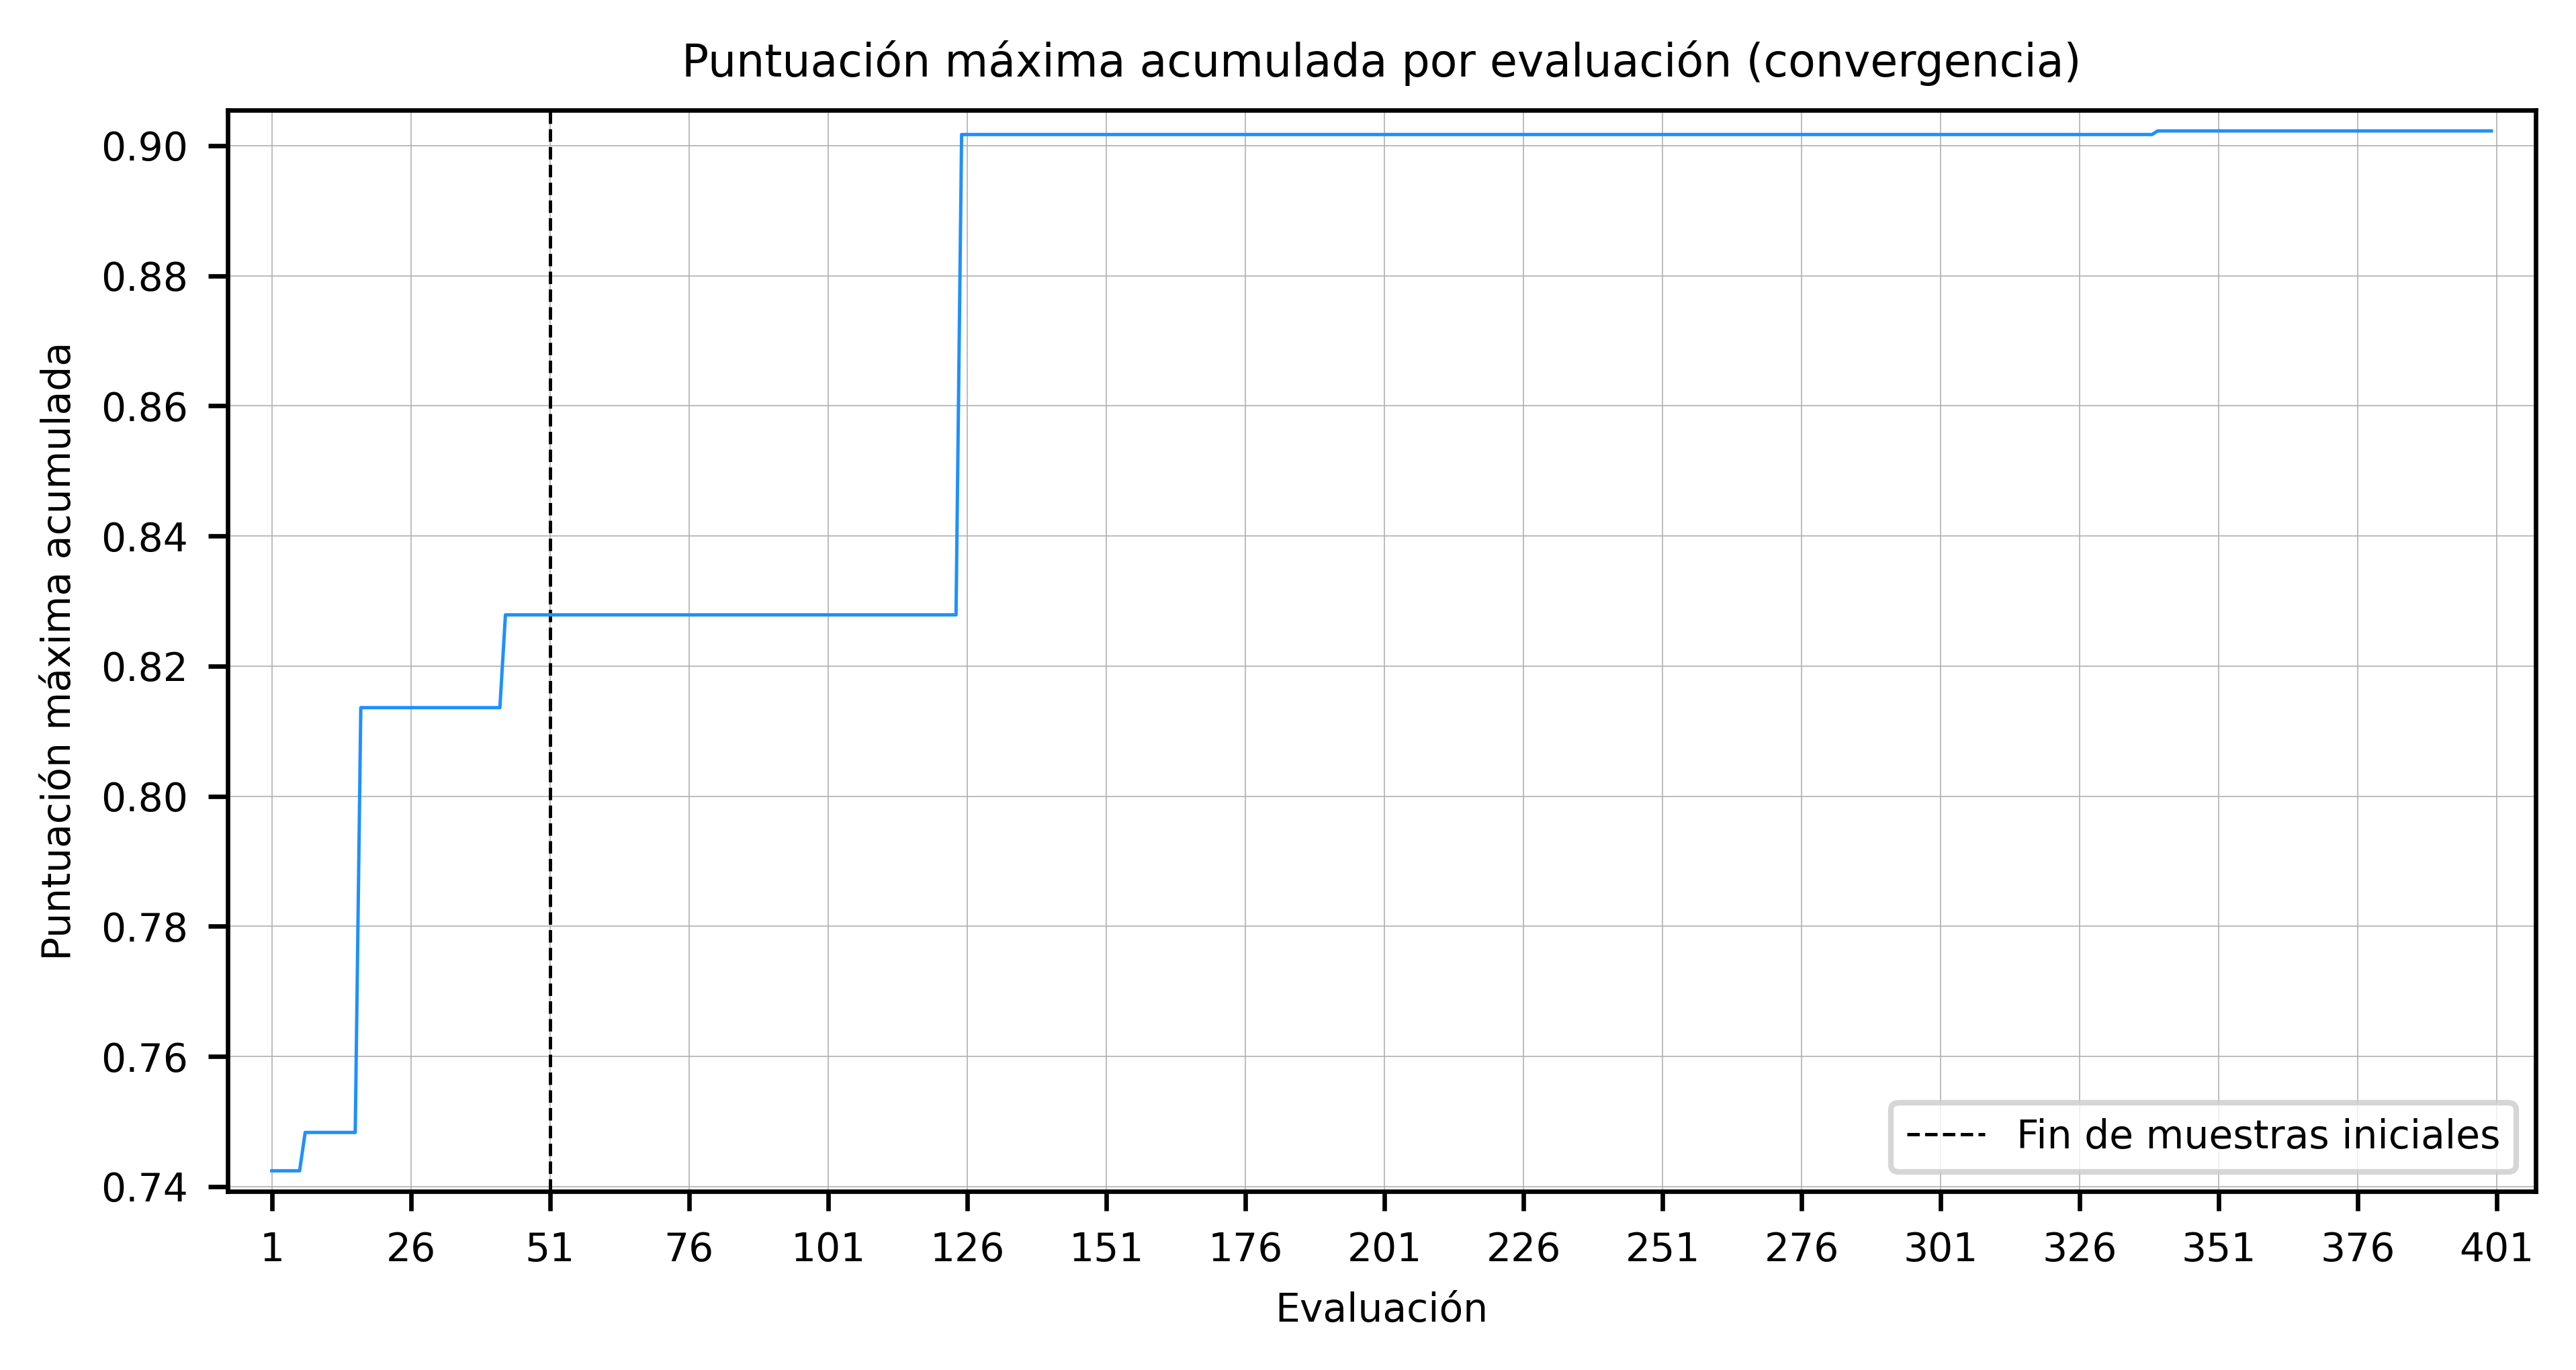
\includegraphics[width=\textwidth, height=\textheight, keepaspectratio]{bo_history_rtxi_syn_model_ifast_islow_antiphase_acc_max}
\end{frame}


\begin{frame}{Resultados implementación \textit{online}: convergencia para fase}
    \centering
    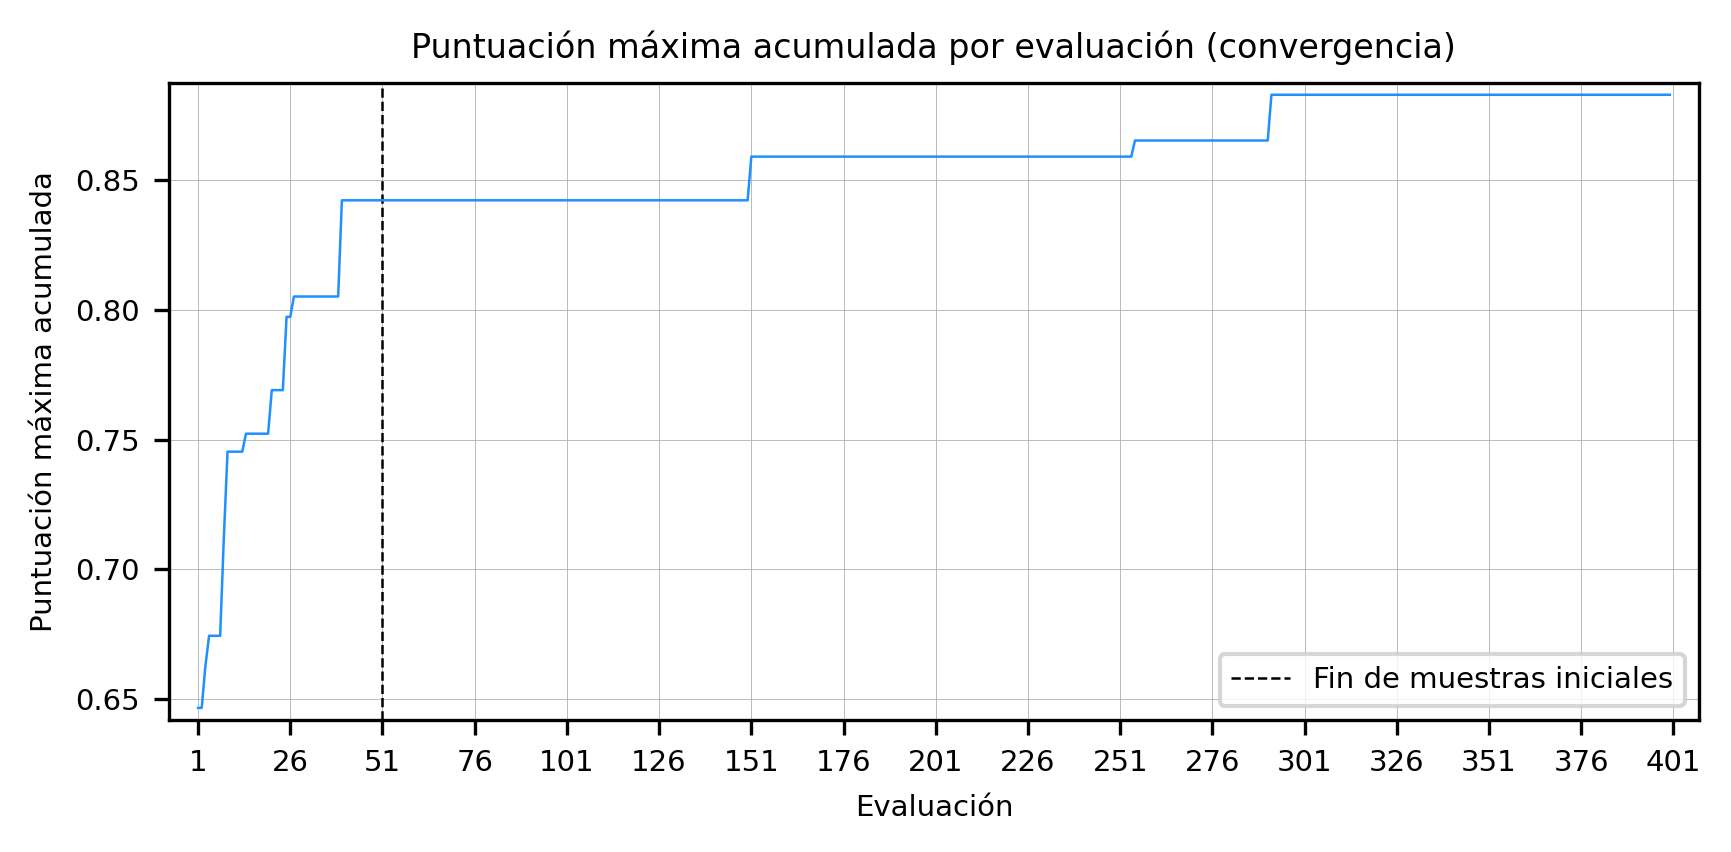
\includegraphics[width=\textwidth, height=\textheight, keepaspectratio]{bo_history_rtxi_syn_model_ifast_islow_phase_acc_max}
\end{frame}


\begin{frame}{Resultados implementación \textit{online}: dinámica result. para antifase}
    \centering
    \vspace{-0.3em}
    \begin{columns}
        \begin{column}{0.6\textwidth}
            \centering
            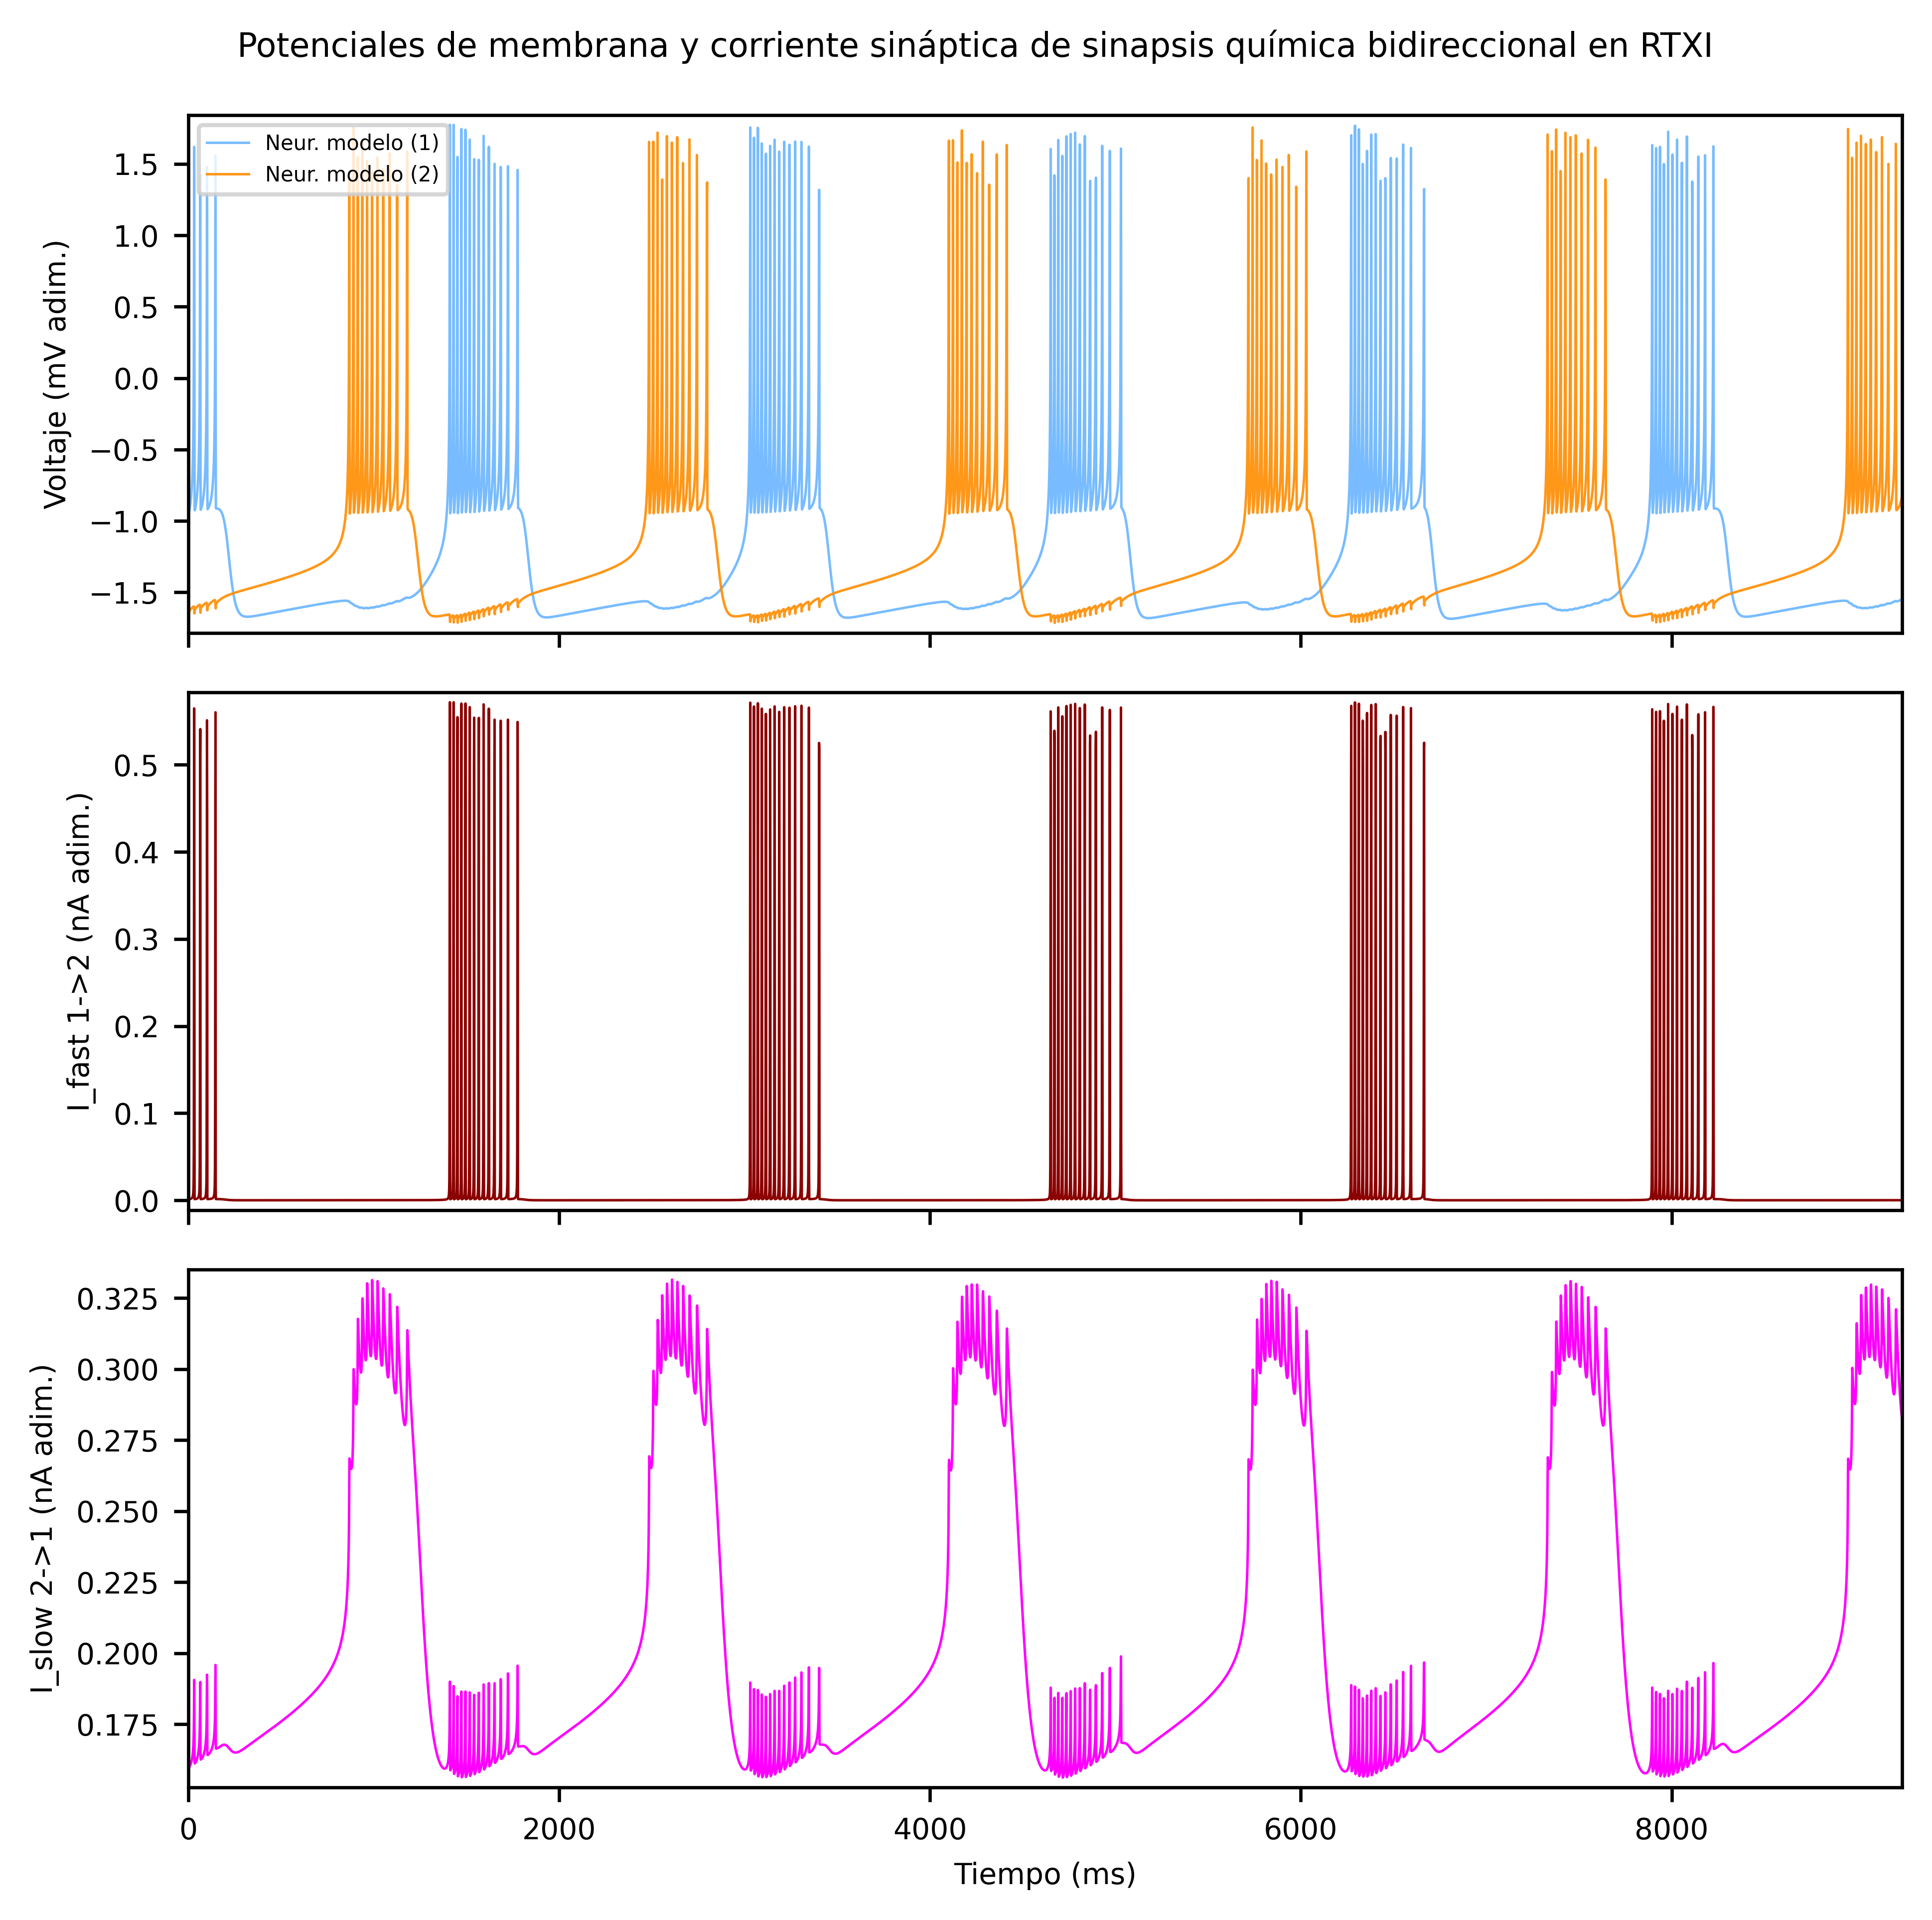
\includegraphics[width=\textwidth, height=0.92\textheight, keepaspectratio]{rtxi_syn_model_ifast_islow_antiphase}
        \end{column}
        \begin{column}{0.4\textwidth}
            \textbf{Rangos de corrientes objetivo}:
            \begin{itemize}
                \item $\boldsymbol{I_{\mathrm{fast}}}$: $\boldsymbol{[0{,}0; 0{,}6]}$ u. a.
                \item $\boldsymbol{I_{\mathrm{slow}}}$: $\boldsymbol{[0{,}2; 0{,}8]}$ u. a.
            \end{itemize}
        \end{column}
    \end{columns}
\end{frame}


\begin{frame}{Resultados implementación \textit{online}: dinámica result. para fase}
    \centering
    \vspace{-0.3em}
    \begin{columns}
        \begin{column}{0.6\textwidth}
            \centering
            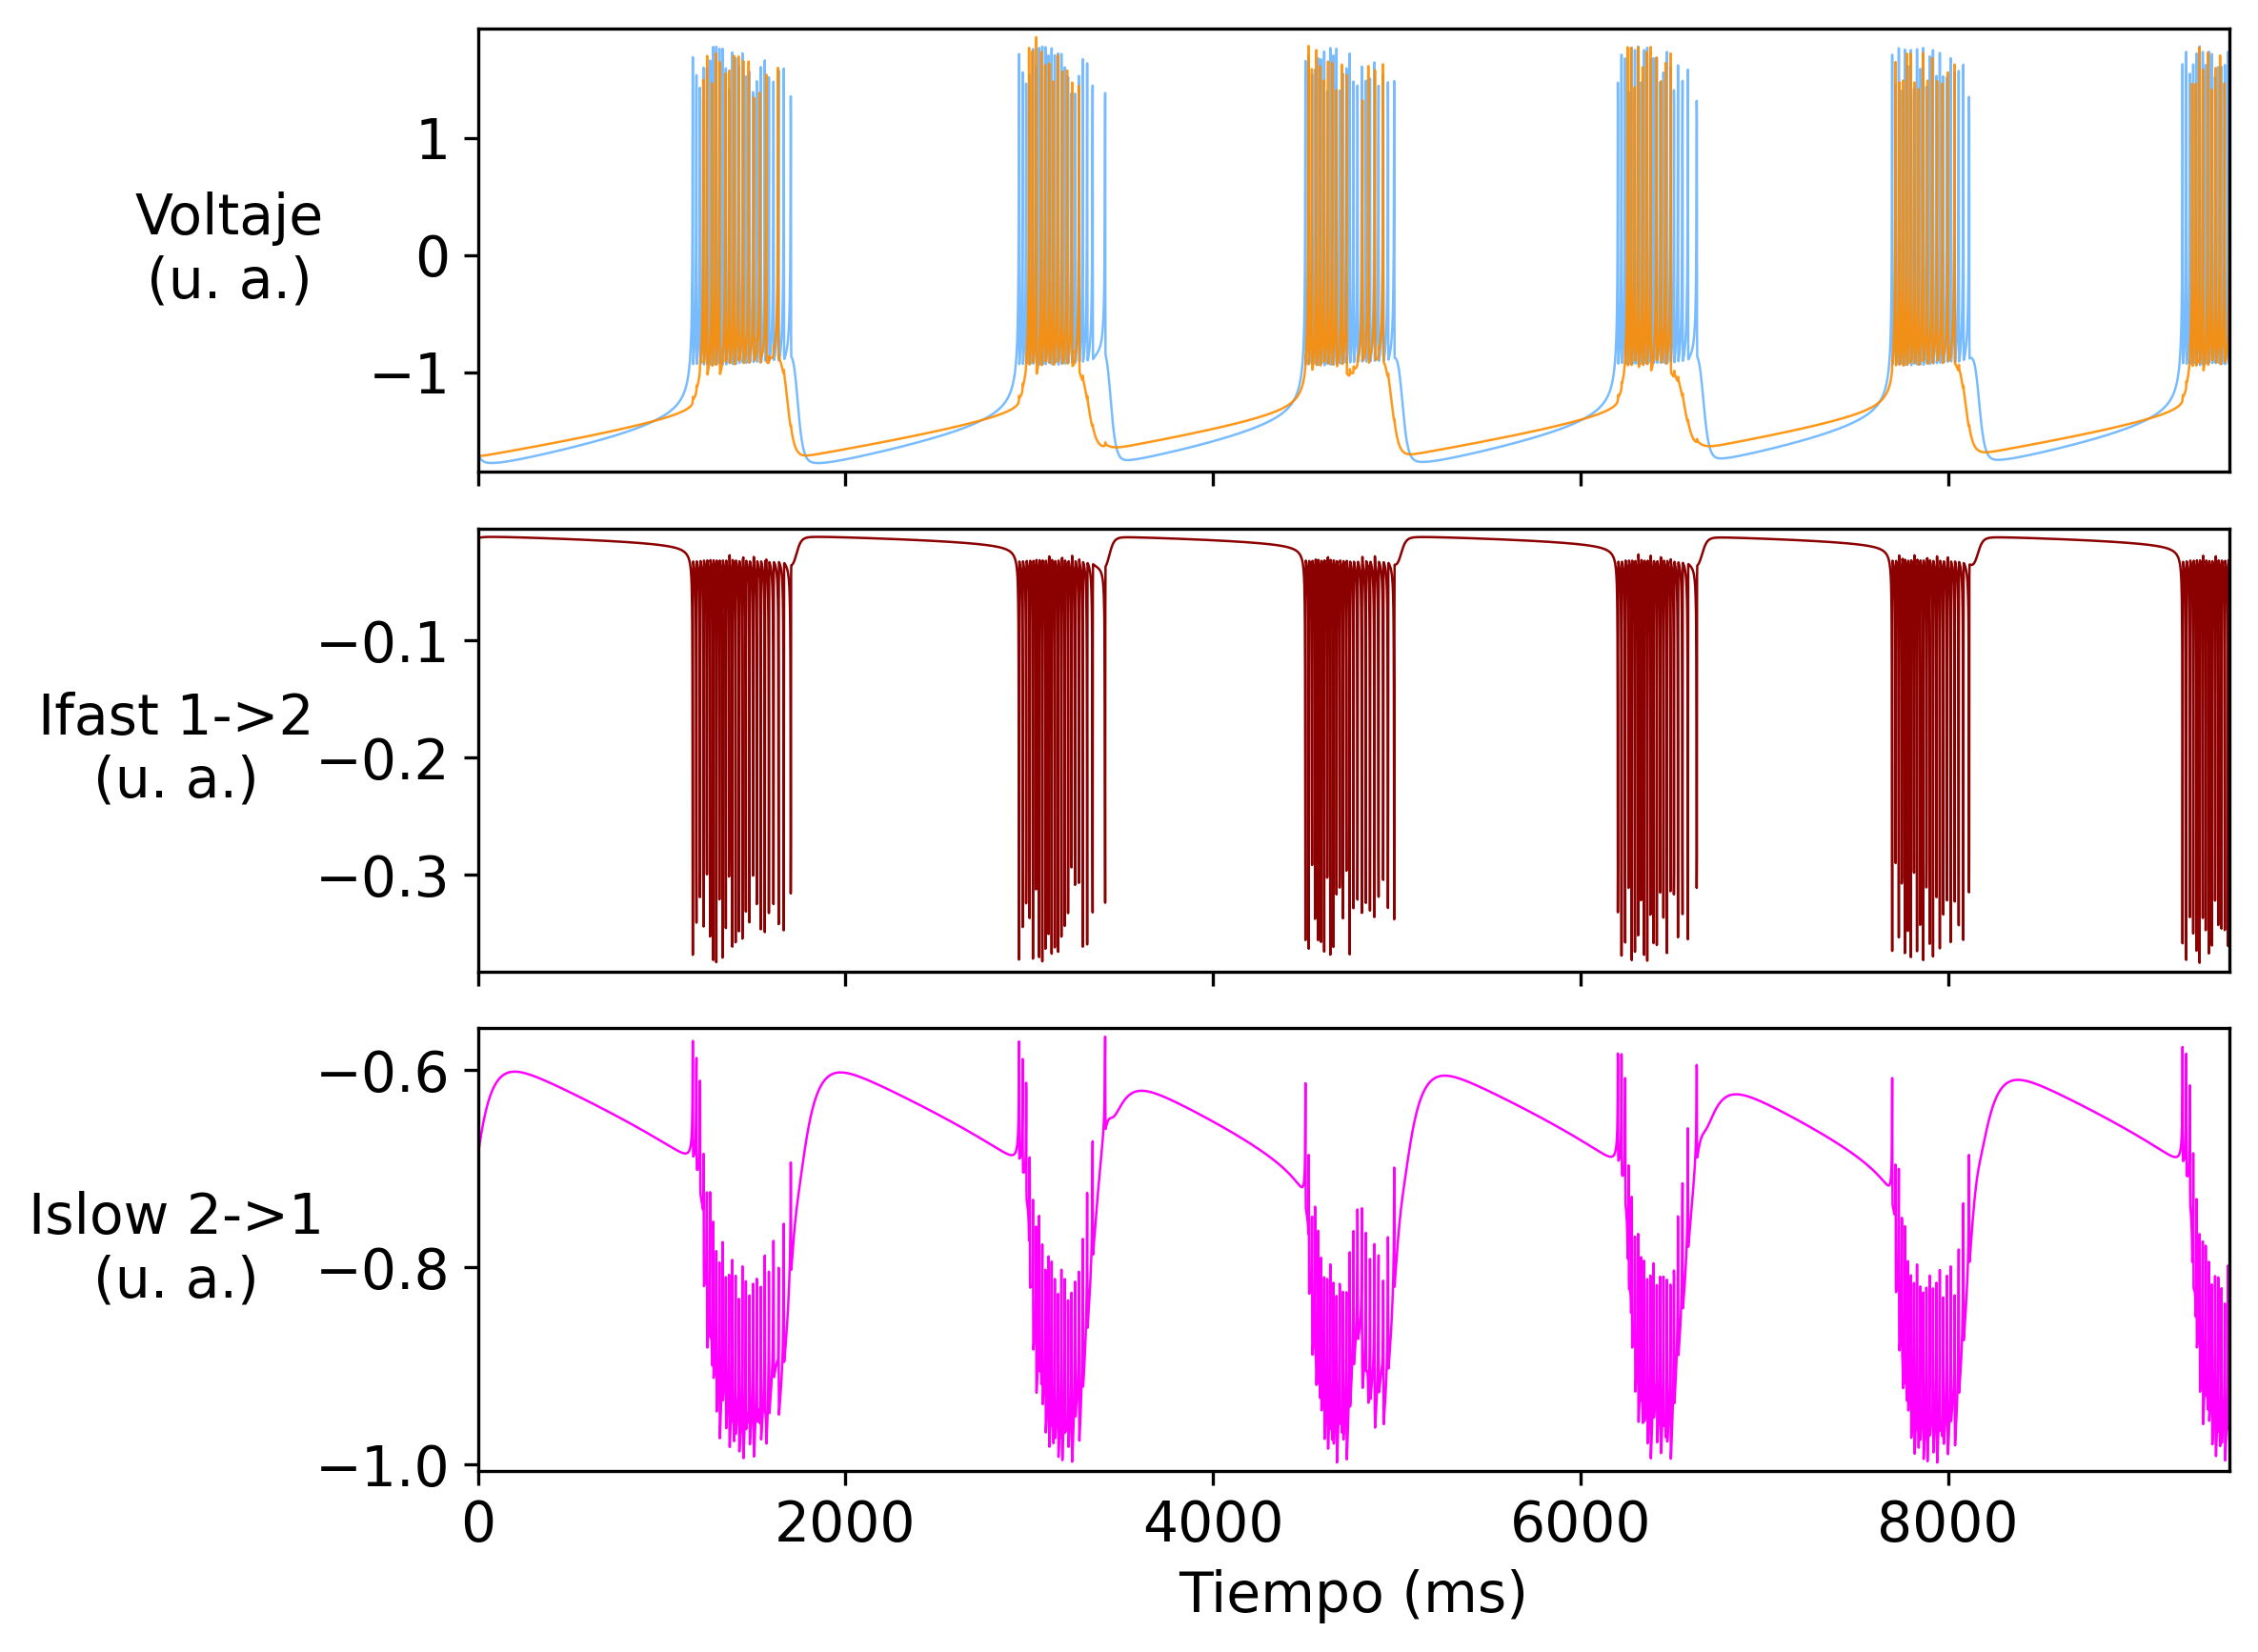
\includegraphics[width=\textwidth, height=0.92\textheight, keepaspectratio]{rtxi_syn_model_ifast_islow_phase}
        \end{column}
        \begin{column}{0.4\textwidth}
            \textbf{Rangos de corrientes objetivo}:
            \begin{itemize}
                \item $\boldsymbol{I_{\mathrm{fast}}}$: $\boldsymbol{[-1{,}0; -0{,}0]}$ u. a.
                \item $\boldsymbol{I_{\mathrm{slow}}}$: $\boldsymbol{[-1{,}4; -0{,}4]}$ u. a.
            \end{itemize}
        \end{column}
    \end{columns}
\end{frame}

\begin{frame}{Resultados implementación \textit{online}: tiempos}
    $\boldsymbol{< 16}$ \textbf{min.} $\to$ \textbf{viable}
\end{frame}


\section{Conclusiones}



\begin{frame}{Conclusiones}
    \begin{itemize}
        \item Los \textbf{objetivos se han cumplido}:
              \begin{itemize}
                  \item[] Implementaciones \textbf{\textit{offline} y \textit{online}} (\textbf{BO y sus configs + configs. de espacio de búsqueda + función de eval. + configs. extra})
                        \begin{itemize}
                            \item \textbf{Convergen adecuadamente} y en \textbf{tiempos viables}
                            \item Logran \textbf{corrientes realistas} (reflejan \textbf{\textit{spikes}} y \textbf{onda lenta} de $\boldsymbol{V_{\mathrm{pre}}}$ de forma separada) \textbf{que causen dinámicas de acoplamiento} (fase/antifase)
                        \end{itemize}
                        haciéndolo la \textbf{\textit{online} sin afectar a tiempo real estricto}.\\[0.2em]
                        Ideal para \textbf{circuitos neuronales biohíbridos}.
              \end{itemize}
        \item Código disponible
    \end{itemize}
\end{frame}


\begin{frame}{Conclusiones}
    \textbf{Limitaciones:}
    \begin{itemize}
        \item Módulo de \textbf{RTXI 2.3} $\to$ \textbf{necesaria adaptación para últimas versiones}
        \item \textbf{Imprecisiones menores en extremos} de rango de corriente resultado respecto a objetivo
    \end{itemize}
    \vspace{0.8em}
    \textbf{Trabajo futuro:}
    \begin{itemize}
        \item \textbf{Validación de implementación online con neuronas vivas} (GNB)
        \item Optimizar \textbf{ambas componentes en ambas direcciones} en implementación \textit{online}
        \item Funciones de \textbf{eval. con información temporal más fina}
        \item Adaptación a \textbf{otros modelos} neuronales y sinápticos
    \end{itemize}
\end{frame}


\begin{frame}[plain]
    \centering
    {\LARGE\bfseries\textcolor{azuloscuro}{Muchas gracias por su atención}}\\[2em]
    {\large\textcolor{azuloscuro}{Parametrización del modelo de sinapsis química\\para circuitos neuronales biohíbridos}}\\[2.5em]
    {\normalsize\textcolor{grisoscuro}{Marco Gómez Hernández}}\\[1.0em]
    {\scriptsize\textcolor{grismedio}{Escuela Politécnica Superior — Universidad Autónoma de Madrid}}\\[1.4em]
    {\small\textcolor{grismedio}{Tutor: Pablo Varona Martínez}}
\end{frame}

\end{document}
